%
% some useful macros
%
\newcommand{\fix}[1]{\textcolor{red}{\texttt{#1}}} % command for comments 
%\newcommand{\fix}[1]{} % remove all comments

\newcommand{\CPP}{C\nolinebreak\hspace{-.05em}\raisebox{.4ex}{\tiny\bf +}\nolinebreak\hspace{-.10em}\raisebox{.4ex}{\tiny\bf +}}

%\subsection{Software}

More than 15 years ago the linear collider community has started to develop common software
tools to facilitate the development and optimization of detector concepts based on realistic
simulations of physics interactions. These software tools eventually led to the creation of
a common software ecosystem called \emph{iLCSoft}~\cite{bib:ilcsoft}.
The \emph{iLCSoft} tools are used by both ILC detector concepts as well as by CLIC
and partly by CEPC and FCC.

From the start, a strong emphasis has been placed on developing flexible and generic tools
that can easily be applied to other experiments or new detector concepts. 
This approach of developing common tools wherever possible has helped considerably in
leveraging the limited manpower and putting the focus on algorithm development that
is crucial for the physics performance. 

In the next sections we will introduce the most relevant tools and algorithms and
describe their design and performance, thereby following the natural flow of data processing
from generated 4-vectors to high level physics objects.


%\subsubsection{Core Software Tools}
\subsection{\label{sub:sw-core-tools}Core Software Tools}

The foundation for the development of common software was laid with LCIO~\cite{Gaede:2003ip}, the
event data model (EDM) and persistency tool for linear collider studies. At the core of LCIO is a hierarchical
EDM for any particle physics experiment, as shown in Fig.\ref{fig:lcio_edm}.
%%%%%%%%%%%%%%%%
\begin{figure}
\begin{center}
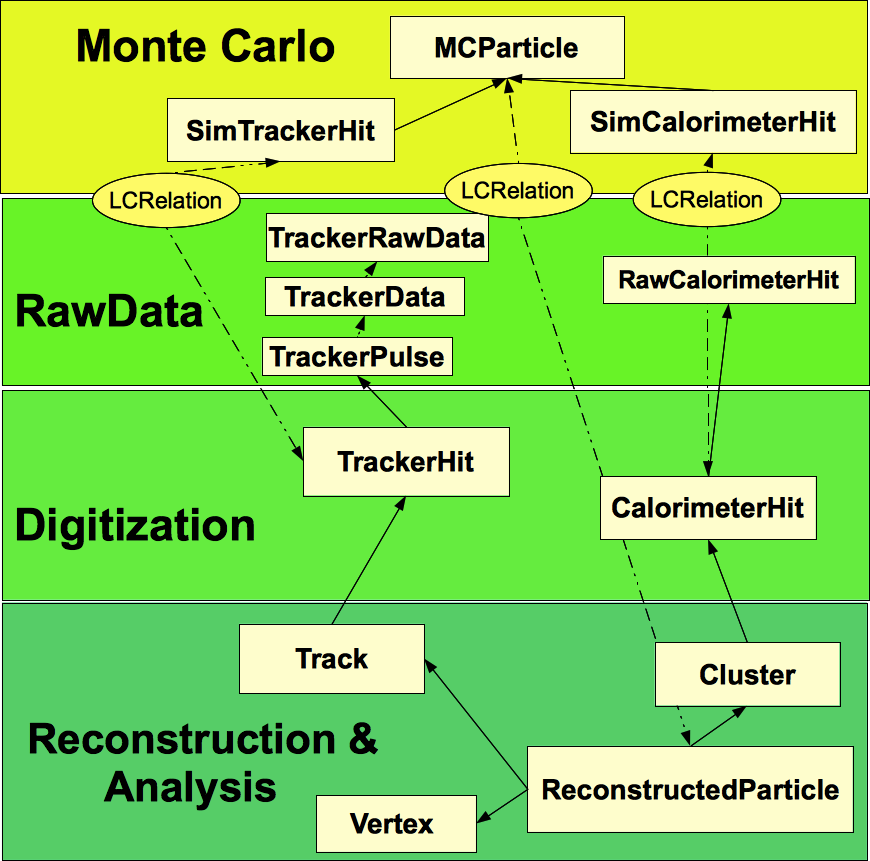
\includegraphics[width=0.60\hsize]{chapters/figures/lcio_edm_schema.png}
\end{center}
\caption{Schematic view of the hierarchical EDM in LCIO.}
\label{fig:lcio_edm}
\end{figure}
%%%%%%%%%%%%%%%%%
It provides data classes for all phases of the event processing, starting from Monte Carlo truth information,
over raw data and digitization to the final reconstruction and analysis. Objects at higher levels of the processing
point back to the lower level constituting objects. As a specific design decision, there are no pointers back to the
Monte Carlo truth but these can be added if needed using dedicated generic LCRelation objects.
These relation objects can be used to create many-to-many relations between arbitrary types in the EDM.
A special class LCGenericObject holds user defined data in named vectors of types int, float and double.
This feature is used in many test beams for conditions data and raw data from the DAQ.
LCIO provides APIs in \CPP, Java and Fortran, where today \CPP\ is used almost exclusively.


The \CPP\ application framework Marlin~\cite{Gaede:2006pj} provides an easy to use environment for developing software
modules on all levels of processing and uses LCIO as its transient data format, i.e. all data that is read in or created
by a software module (called \emph{Processor}) are stored in the \emph{LCEvent} class from LCIO. Marlin processors
are self-documenting and controlled via xml-steering files. As processors have well defined input and output data, Marlin
provides a \emph{"Plug-And-Play"} environment, where any specific algorithm can easily be exchanged with another
equivalent implementation for direct comparisons and benchmarking.


The generic detector description toolkit DD4hep~\cite{Frank:2014zya,Frank:2015ivo} provides a powerful tool for describing
the detector geometries, materials and readout properties. DD4hep follows a modular component based approach and provides
interfaces to full simulations with Geant4~\cite{Agostinelli:2002hh} via DDG4, to reconstruction programs via DDRec and to
conditions data and alignment with DDCond and DDAlign respectively, see Fig.\ref{fig:dd4hep}.
%%%%%%%%%%%%%%%%
\begin{figure}
\begin{center}
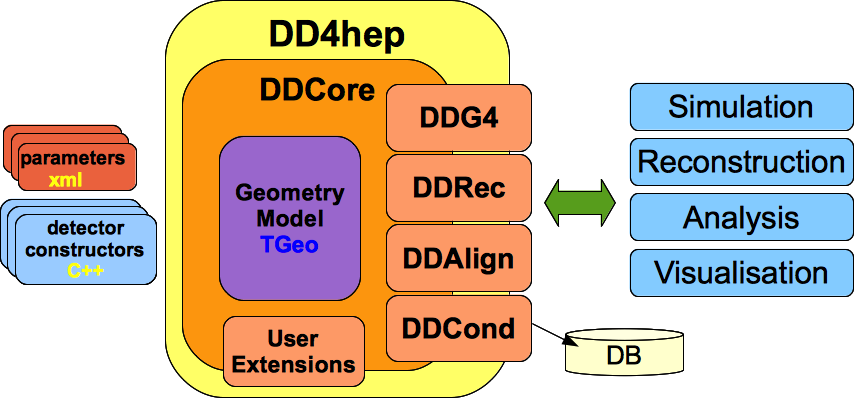
\includegraphics[width=0.90\hsize]{chapters/figures/dd4hep_simple_schema.png}
\end{center}
\caption{Schematic view of DD4hep with its main components and interfaces.}
\label{fig:dd4hep}
\end{figure}
%%%%%%%%%%%%%%%%%
DD4hep is an excellent example for the development of generic software tools for the wider HEP community and was one of the
first incubator projects adopted by the Hep Software Foundation. While it was developed to address the needs of the linear
collider community, it is now used by several other projects and is under evaluation by LHC experiments.


%\subsubsection{Event Generators}
\subsection{\label{sub:sw-generators}Event Generators}

Both detector concepts have created large, realistic Monte Carlo samples with the full Standard Model physics as well as various
BSM scenarios that have been used for the physics analyses presented in the following sections.
In a first step, large generator samples with $e^+e^-$-events are created with the Whizard~\cite{Kilian:2007gr} event generator.
Whizard uses tree-level matrix elements and loop corrections to generate events with the final state partons and leptons
based on a realistic beam energy spectrum, the so called \emph{hard sub-process}. The hadronization into the visible final state
is performed with Pythia~\cite{Sjostrand:2006za} tuned to describe the LEP data.

The input spectrum is created with Guinea-Pig~\cite{Schulte:1998au}, a dedicated simulation program for computing
beam-beam interactions at linear colliders. The two dominating effects of the strong beam-beam interactions are the 
beamstrahlung leading to the available luminosity spectrum (see Fig~\ref{fig:lumi_spectrum}) and the creation of
incoherent $e^+e^-$-pairs that are the source of the dominating background at the ILC. These electrons and positrons
are predominantly created in a forward cone as shown in Fig~\ref{fig:pair_bg}. It is this cone that restricts the minimal
allowed radius of the innermost layer of the vertex detector.

%%%%%%%%%%%%%%%%
\begin{figure}
\begin{center}
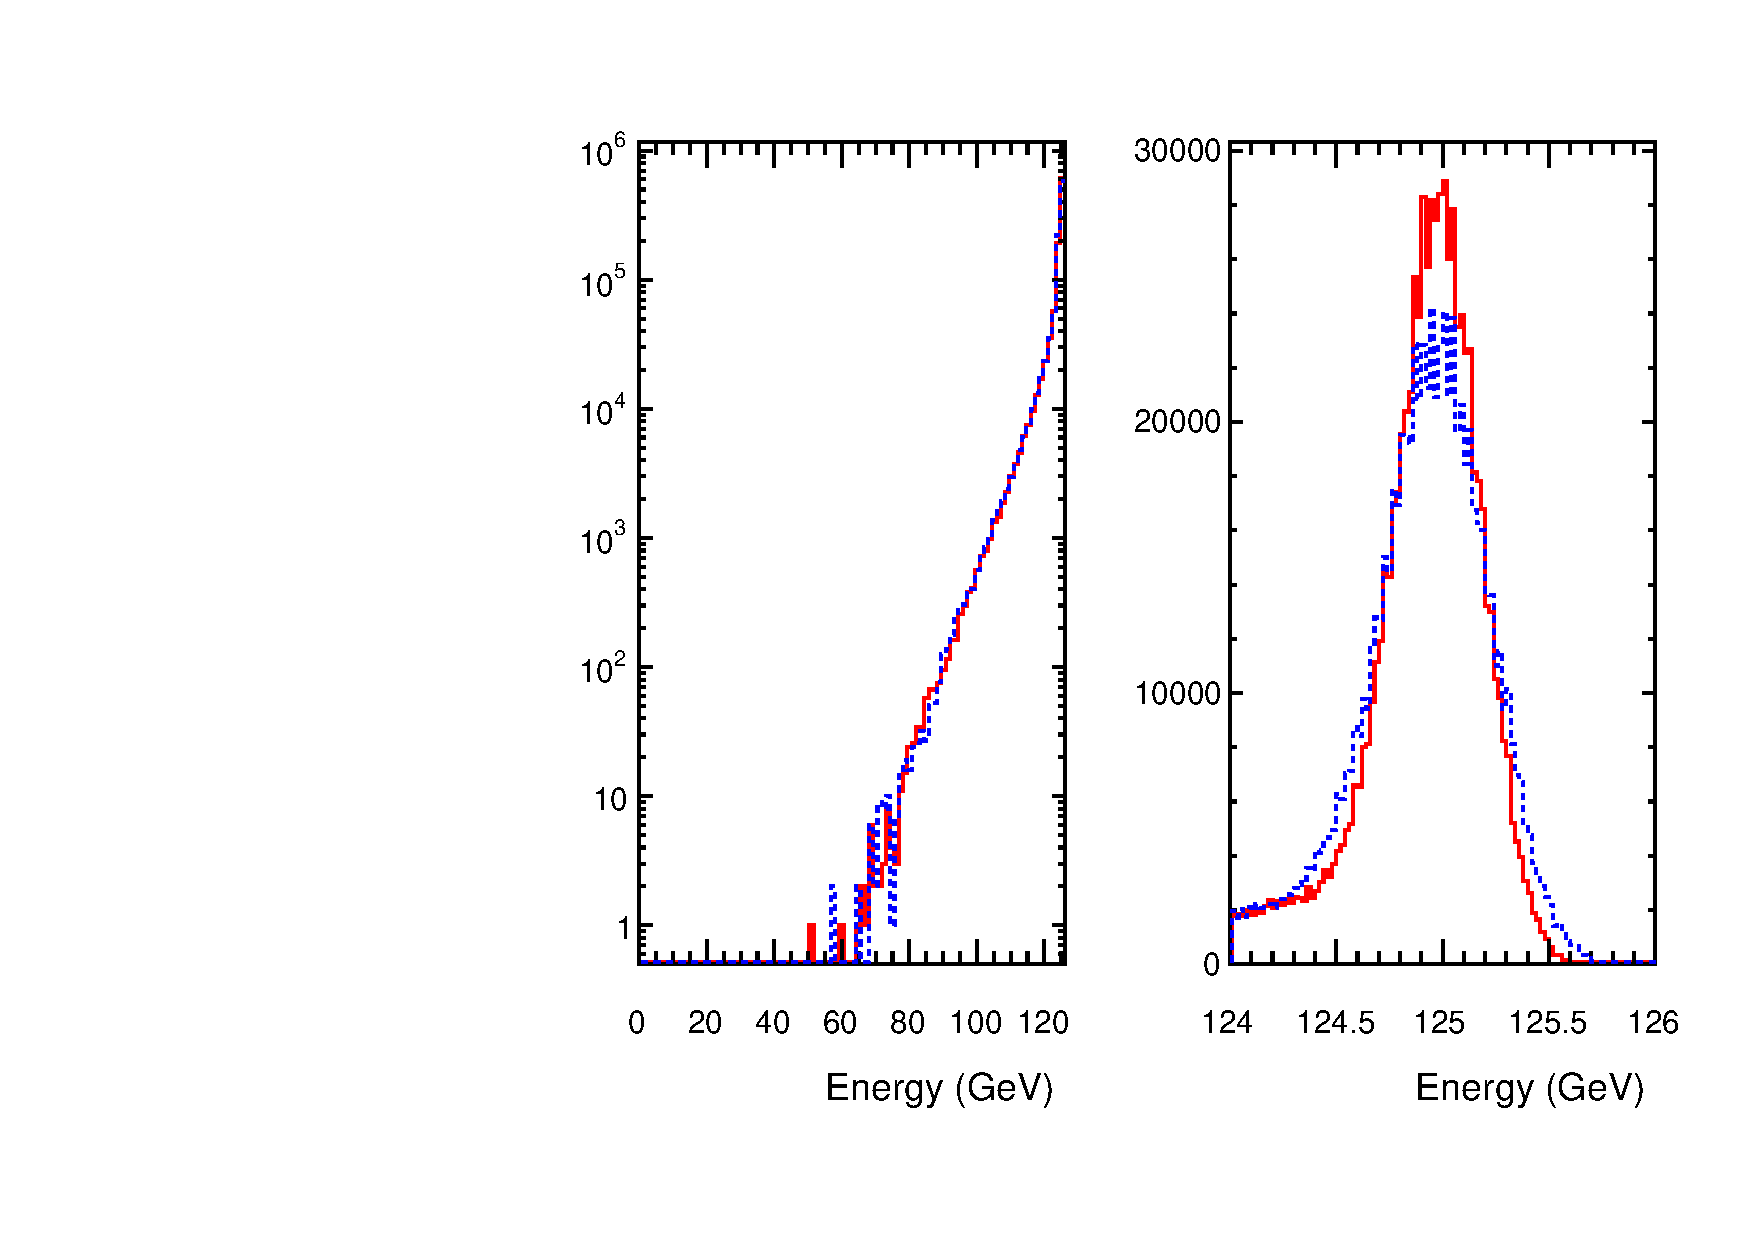
\includegraphics[width=1.\hsize]{chapters/figures/beam_spectrum_gp_250Gev_SetA.pdf}
\end{center}
\caption{Beam energy spectra for $\sqrt{s}=250~\rm{GeV}$ Set-A, created with GuineaPig (blue-dashed: $e^-$, red-solid $e^+$).}
\label{fig:lumi_spectrum}
\end{figure}
%%%%%%%%%%%%%%%%%

%%%%%%%%%%%%%%%%
\begin{figure}
\begin{center}
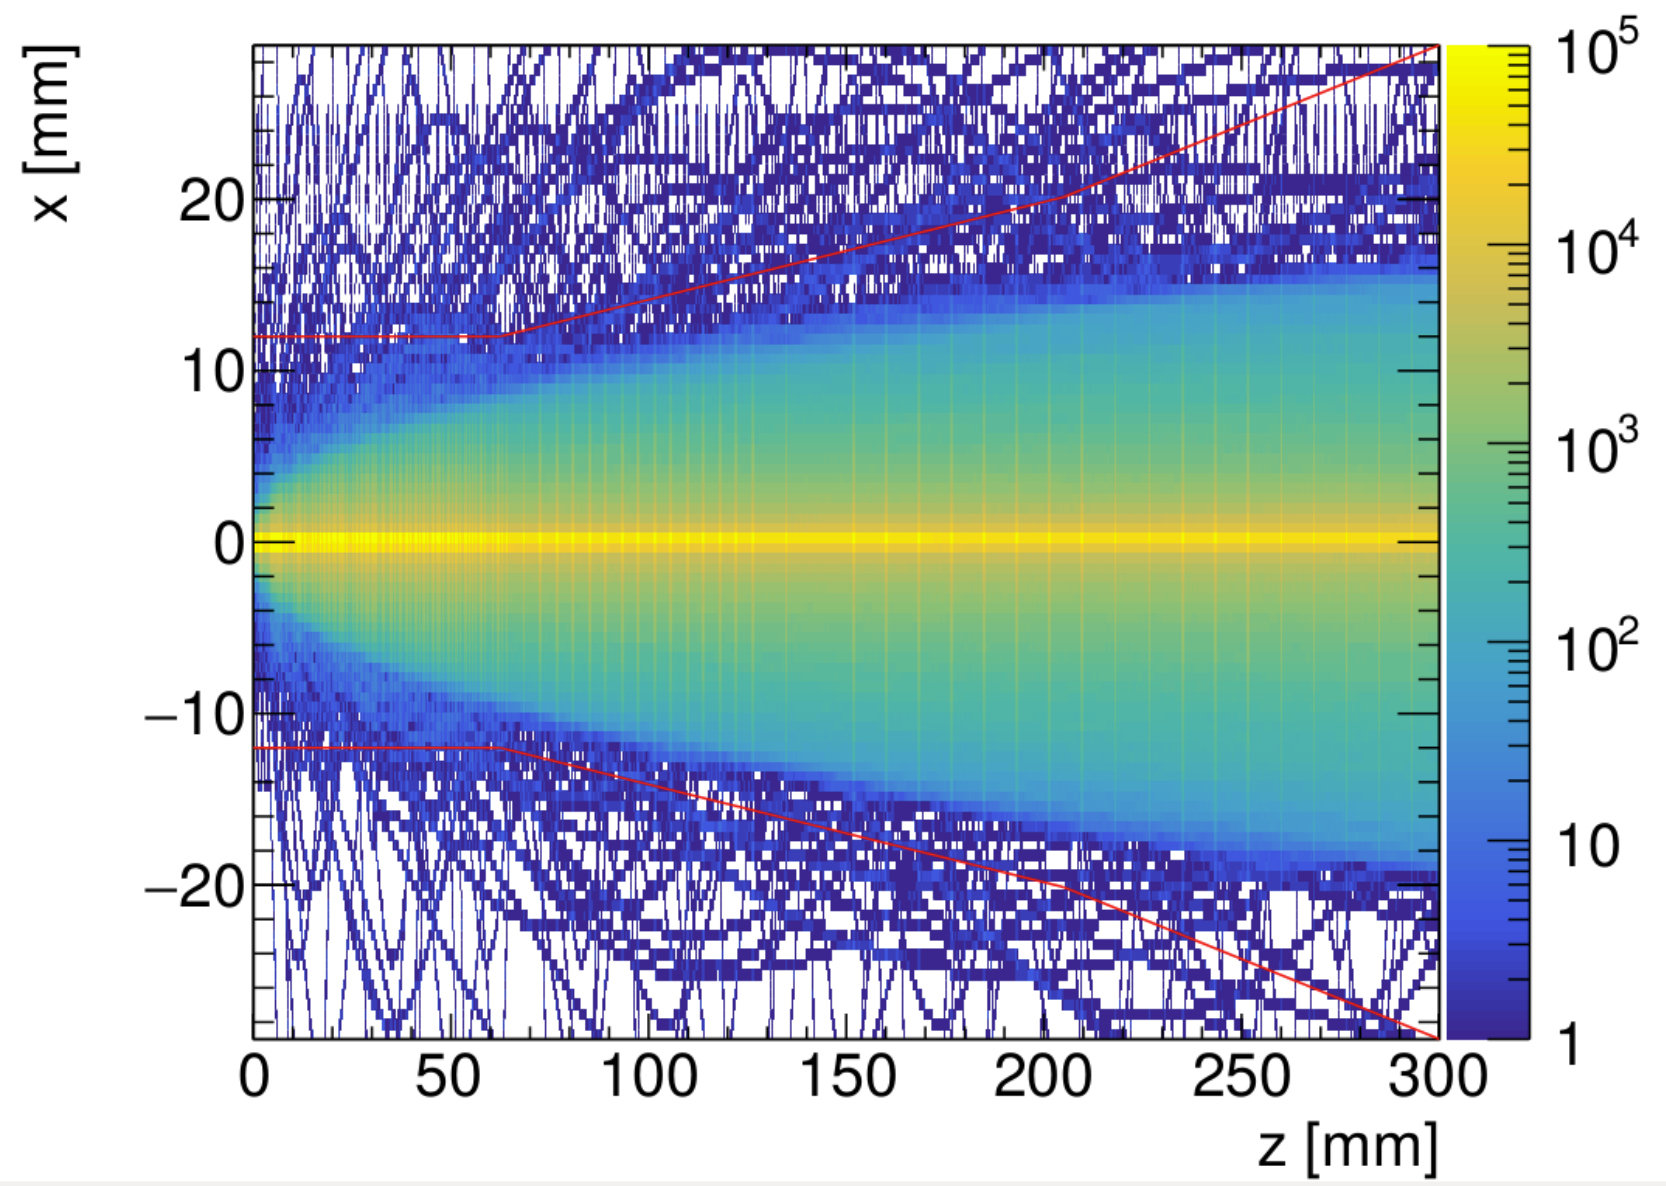
\includegraphics[width=0.90\hsize]{chapters/figures/pair_bg_cone_SiD.png}
\end{center}
\caption{Cone of background from incoherent $e^+e^-$-pairs, generated with Guinea-Pig and simulated in the 5 T B-field of the SiD
  detector (from~\cite{Schutz:2017ihd}).}
\label{fig:pair_bg}
\end{figure}
%%%%%%%%%%%%%%%%%

Another source of background at the ILC are $\gamma \gamma \rightarrow hadrons$ events, due to bremsstrahlung and beamstrahlung photons.
These type of events are generated for $\gamma \gamma$ cms-energies from $300~\rm{MeV~to} ~2~\rm{GeV}.$ with a dedicated generator based
on ~\cite{Chen:1993dba}, for higher energies Pythia is used.


%\subsubsection{Simulation}
\subsection{\label{sub:sw-sim}Simulation}

Both detector concepts have adopted DD4hep for describing their detector simulation models and use \emph{ddsim}, a python application that
is based on the DDG4 component, providing a gateway to full simulations with Geant4.
In DD4hep the detector geometry is implemented in dedicated \CPP modules for every subdetector and the actual parameters with dimensions
and materials are provided via compact xml-files. A large palette of predefined sub-detector drivers exists in DD4hep, allowing for an
easy implementation of a new detector concept by providing suitable compact files.
A dedicated software package lcgeo~\cite{bib:lcgeo}, which is shared by SiD, ILD and CLICdp, contains all subdetector drivers for the
detector concepts under study by these groups, together with the corresponding compact parameter files.

%%%%%%%%%%%%%%%%
\begin{figure}
\begin{center}
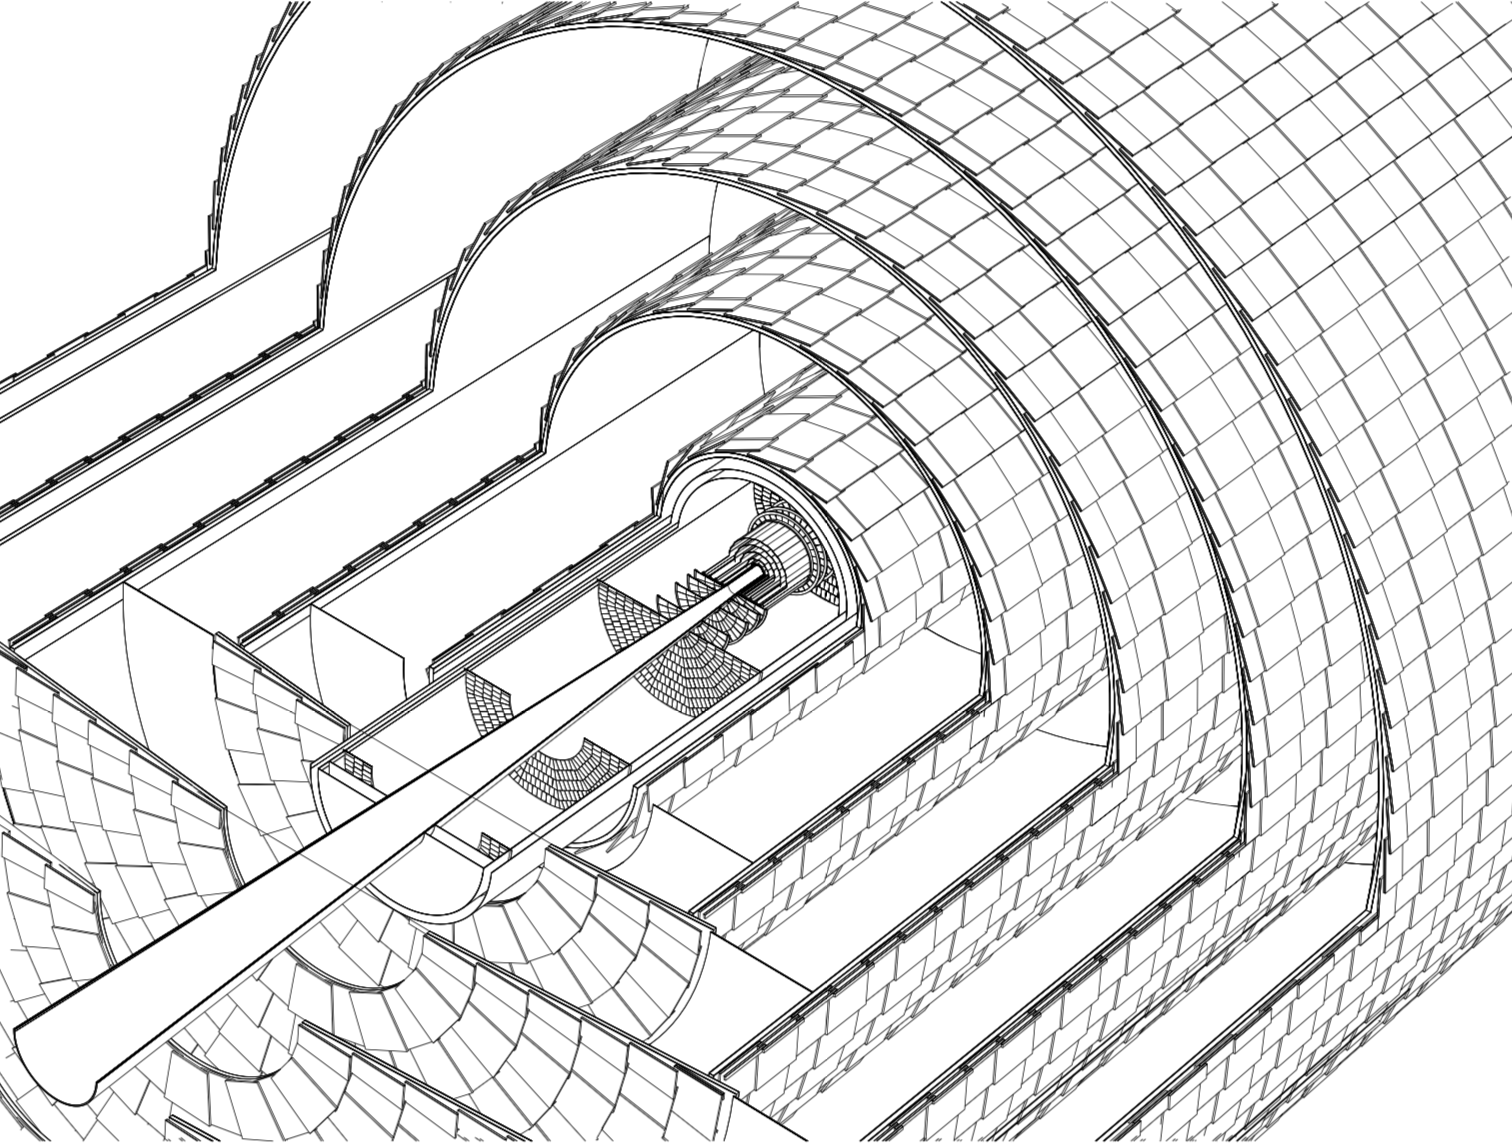
\includegraphics[width=0.80\hsize]{chapters/figures/SiD_tracker_simmodel.png}
\end{center}
\caption{Cut-away view of the tracking system as implemented in the \emph{SIDLOI3} simulation model (from~\cite{Behnke:2013lya}).}
\label{fig:sid_trk}
\end{figure}
%%%%%%%%%%%%%%%%%
Both detector concept groups have invested considerable effort into making their full-simulation models as realistic as possible, by
\begin{itemize}
\item following the exact dimensions and layout of detector elements from engineering models
\item implementing correct material properties
\item implementing precise descriptions of the actual detector technology
\item adding realistic amounts of dead material from supports and services, such as cables and cooling pipes
\item introducing realistic gaps and imperfections into the subdetectors
\end{itemize}
Care has been taken to include realistic material estimates in particular in the tracking region where
the material budget has a direct impact on the detector performance.
Figure~\ref{fig:sid_trk} shows the tracking detector as implemented for the SiD simulation model.
%%%%%%%%%%%%%%%%
\begin{figure}
\begin{center}
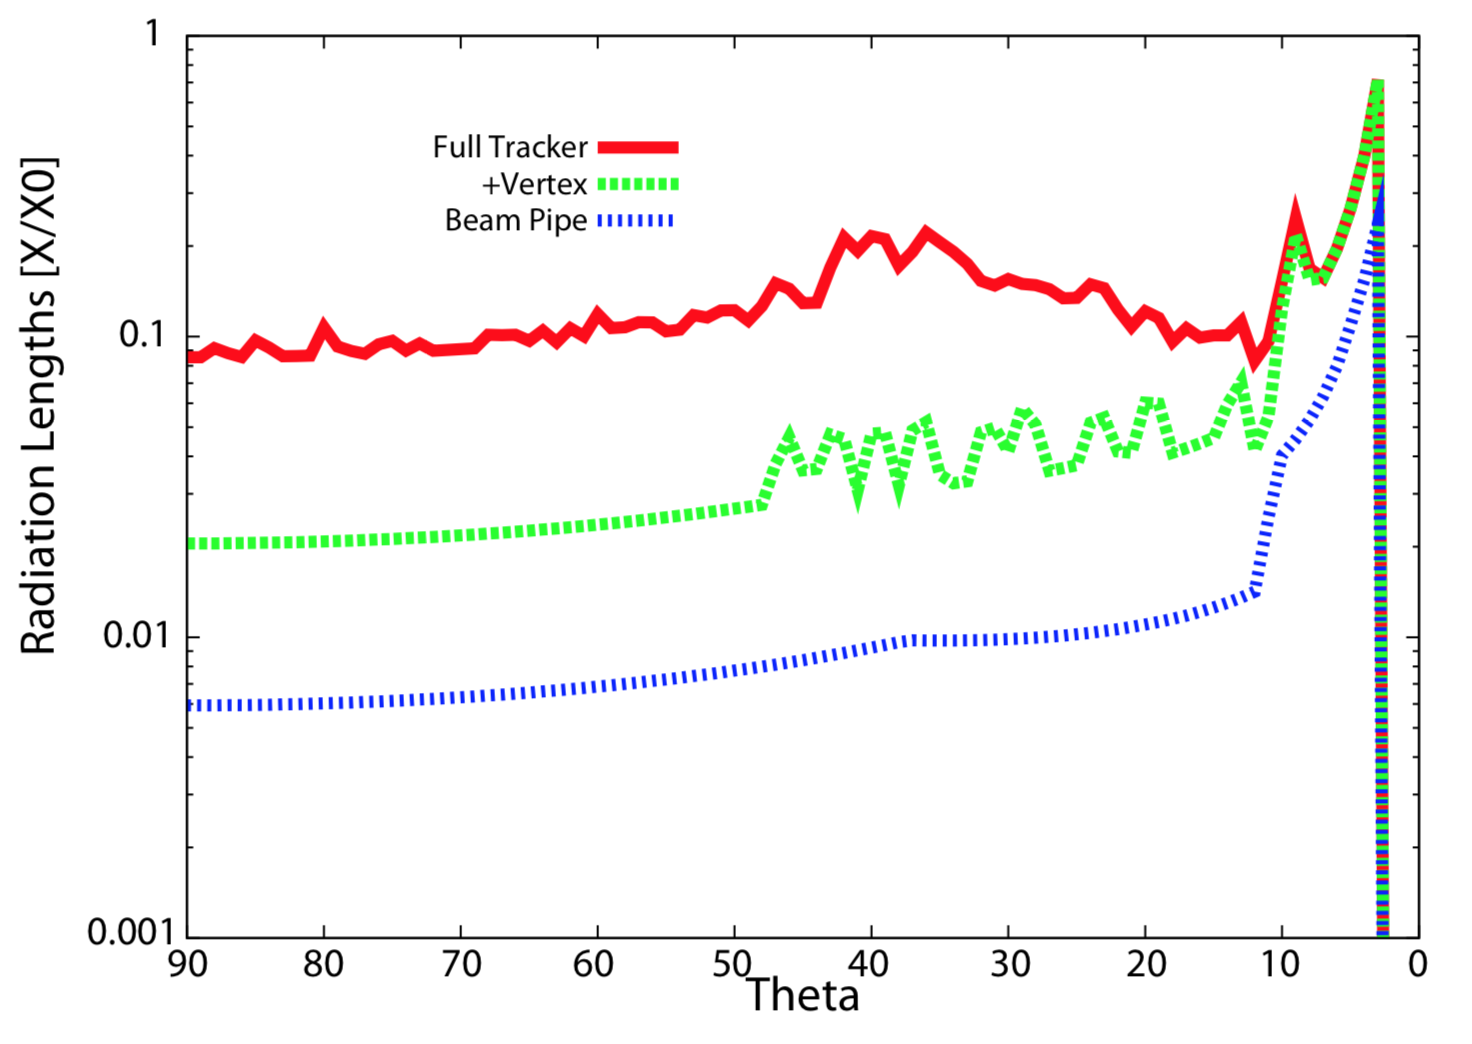
\includegraphics[width=0.80\hsize]{chapters/figures/SiD_material_budget_tracker.png}
\end{center}
\caption{Resulting radiation lengths of the tracking detectors in the \emph{SIDLOI3} simulation model (from~\cite{Behnke:2013lya}).}
\label{fig:sid_mat_budget}
\end{figure}
%%%%%%%%%%%%%%%%%
%%%%%%%%%%%%%%%%
\begin{figure}
\begin{center}
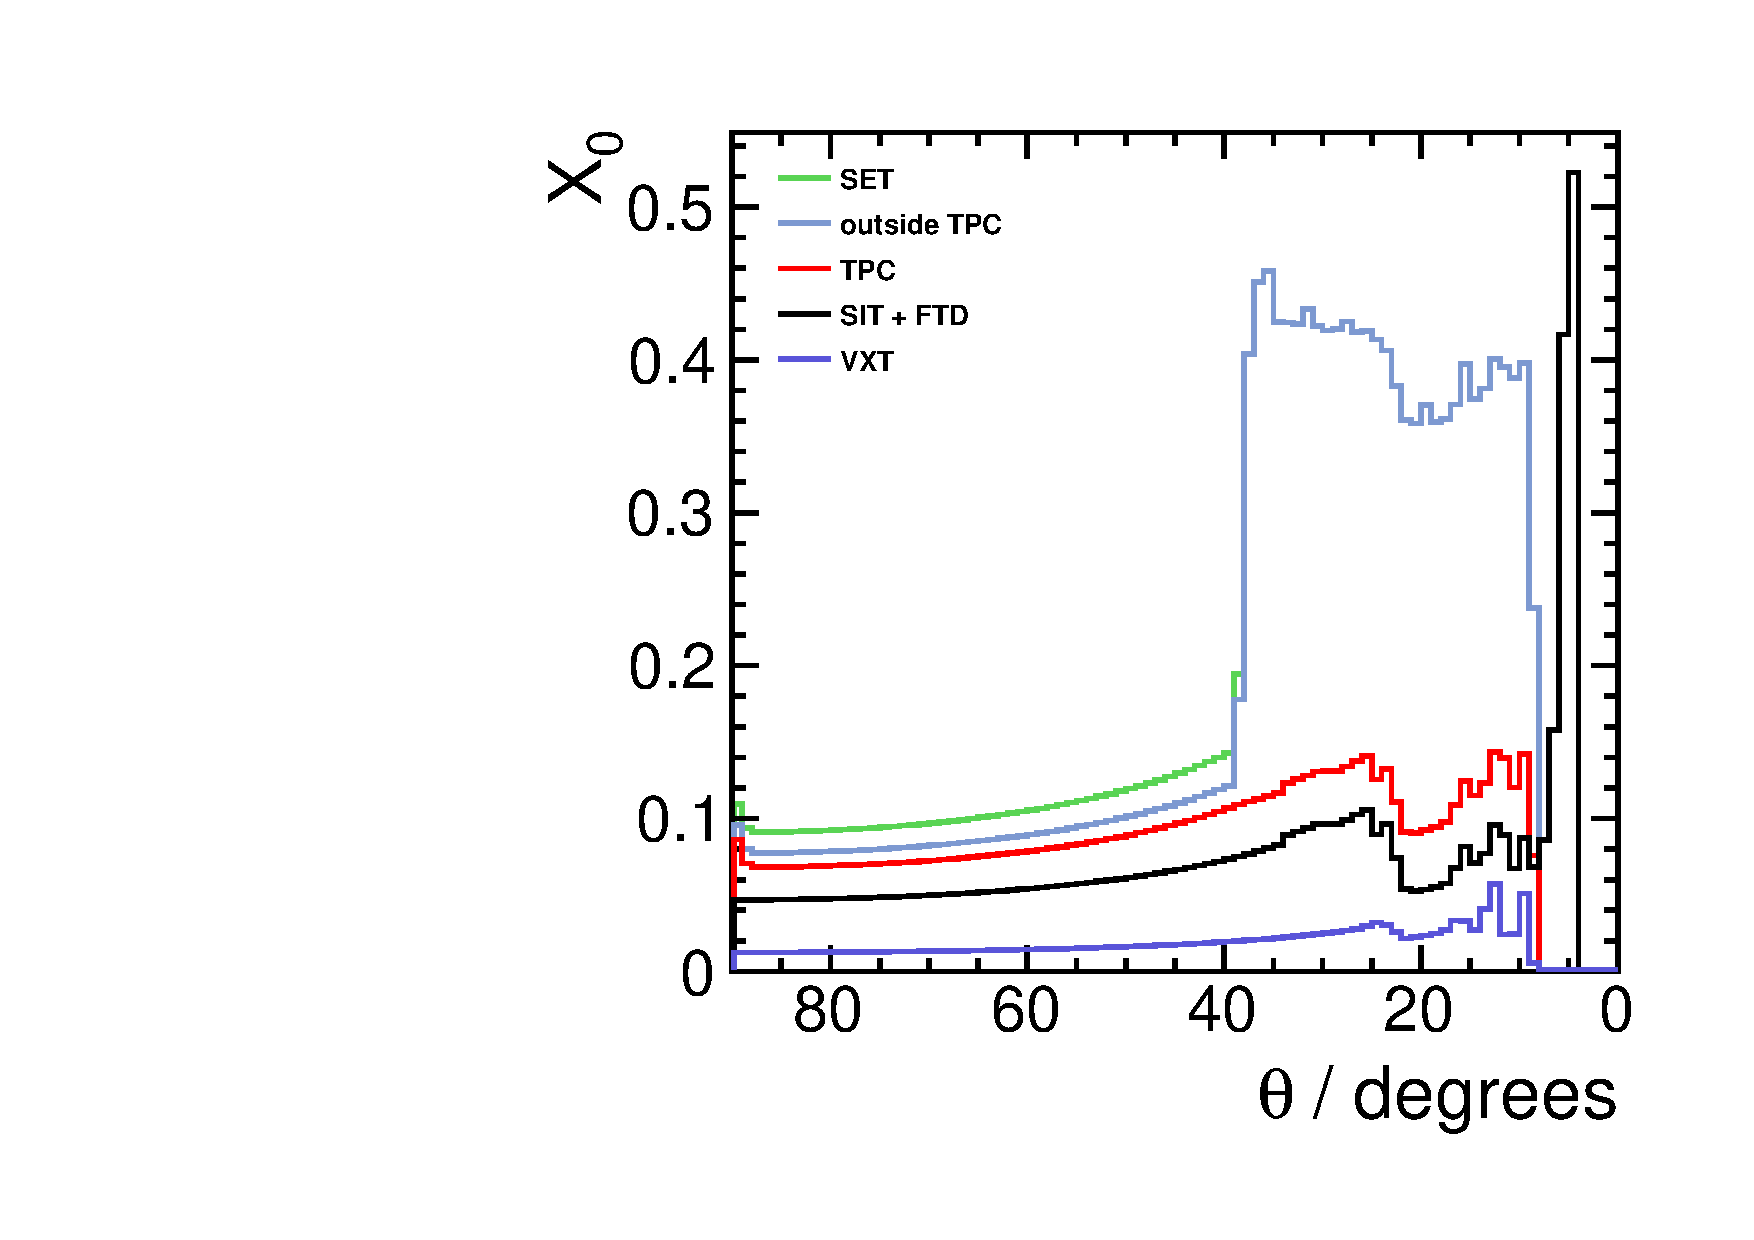
\includegraphics[width=0.80\hsize]{chapters/figures/ILD_material_budget_tracker.pdf}
\end{center}
\caption{Resulting radiation lengths of the tracking detectors in the \emph{ILD\_o1\_v05} simulation model (from~\cite{Behnke:2013lya}).}
\label{fig:ILD_mat_budget}
\end{figure}
%%%%%%%%%%%%%%%%%
The average material budget in the tracking volume of the simulation models is shown in Figures~\ref{fig:sid_mat_budget}
and~\ref{fig:ILD_mat_budget} for SiD and ILD respectively.

Before the two concepts had decided to move to the common geometry description and simulation with DD4hep, they had
implemented their detailed simulation models in Mokka~\cite{MoradeFreitas:2002kj} and slic~\cite{bib:slic}. These models
have been ported into DD4hep preserving all features and dimensions, thus resulting in equivalent simulation results.
Most of the physics analyses in the next sections are based on simulations using these older programs.

The high level of detail in the simulation models as decried above is a key prerequisite for the
realistic understanding of the expected detector performance and the physics reach of the ILC for both detector concepts.


%\subsubsection{Digitzation}
\subsection{\label{sub:sw-digi}Digitzation}

The output of the detailed full simulations with Geant4 from ddsim are \emph{SimTrackerHit} and \emph{SimCalorimeterHit} objects,
that store the deposited energy in the sensitive detector elements, such as silicon wafers and calorimeter cells, together with
the position and pointers to the \emph{MCParticle} that created the energy deposition. In the digitization step, carried out in dedicated
Marlin processors, these hits are converted into \emph{TrackerHit} and \emph{CalorimeterHit} objects,
taking into account all relevant effects from the detector and the readout electronics.

The \emph{SimTrackerHits} contain the exact energy-weighted position of the individual energy depositions in a given sensitive
detector element. For silicon strip-and pixel detectors as well as the ILD-TPC, these positions are smeared according to
resolutions that have been established from test beam campaigns for the different sensor technologies, thereby including effects
from charge sharing, clustering and position reconstruction. Table~\ref{tab:ild_trk_res} shows the point resolution parameters used for ILD.



%-----------------------------------------------------------------------
\begin{table}[htbp]
\renewcommand{\arraystretch}{1.25}

\centering\small
\begin{tabular}{llcl}
\hline
 Subdetector &  \multicolumn{3}{c}{ Point Resolution }  \\
\hline
        VTX    &  $ \sigma_{r\phi,z}  $ & $=$ & $ 2.8 \mu\mathrm{m}$   (layer 1)   \\
               &  $ \sigma_{r\phi,z}  $ & $=$ & $ 6.0 \mu\mathrm{m}$   (layer 2)   \\
               &  $ \sigma_{r\phi,z}  $ & $=$ & $ 4.0 \mu\mathrm{m}$   (layers 3-6)   \\


        SIT    &  $ \sigma_{\alpha_{z}}   $ & $=$ & $ 7.0 \mu\mathrm{m}$    \\
               &  $  \alpha_{z}         $ & $=$ & $ \pm 7.0^\circ $ (angle with z-axis)        \\

        SET    &  $ \sigma_{\alpha_{z}}   $ & $=$ & $ 7.0 \mu\mathrm{m}$    \\
               &  $  \alpha_{z}         $ & $=$ & $ \pm 7.0^\circ $ (angle with z-axis)        \\

       FTD     &  $\sigma_{r}$      & $=$ & $ 3.0 \mu\mathrm{m}$    \\
  \emph{Pixel} &  $ \sigma_{r_\perp}$  & $=$ & $ 3.0 \mu\mathrm{m}$    \\

     FTD       &  $ \sigma_{\alpha_r}   $ & $=$ & $ 7.0 \mu\mathrm{m}$    \\
  \emph{Strip} &  $ \alpha_{r}         $ & $=$ & $ \pm 5.0^\circ $ (angle with radial direction)        \\

       TPC    &  $ \sigma^2_{r\phi} $ & $=$ & $ \bigl( 50^2+900^2\sin^2\phi + \bigl( (25^2/22)\times$  \\
              &                      &     &   $(4T/B)^2\sin\theta\bigr) (z/\mathrm{cm}) \bigr)\,\mu\mathrm{m}^2$  \\
               &  $ \sigma^2_{z}    $ & $=$ & $ (400^2+80^2\times (z/\mathrm{cm})) \,\mu\mathrm{m}^2 $ \\
               &   \multicolumn{3}{c}{ where $\phi$ and $\theta$ are the azimuthal and} \\
               &   \multicolumn{3}{c}{ polar angle of the track direction } \\
\hline
\end{tabular}
\caption[Simulated ILD tracking point resolutions.]{Effective point resolutions as used in the digitization of the ILD tracking detectors.
  The parameterization for the TPC takes into account geometric effects due to the direction of the track with respect to the pad row and
  has been established from test beam data.
        \label{tab:ild_trk_res} }
\end{table}
%-----------------------------------------------------------------------

In the TPC hit digitization, simulated hits that are closer than the established double-hit resolution of 2~mm in $r\phi$ and 5~mm
in $z$ are merged into one. For the silicon detectors this treatment is not necessary, due to the expected low occupancies.

The \emph{SimCalorimeterHits} contain the total energy deposited in each calorimeter cell, together with the individual depositions
from the individual Monte Carlo steps. For scintillating calorimeters Birk's Law, resulting in different light yields for different
particles, is already applied during the simulation. Dedicated digitizers take into account effects of non-uniformity of the light yield
for scintillators as well as cross-talk between neighboring channels. The latter is important in particular for the simulation of
(semi)-digital calorimeters using RPCs and is possible due to the availability of the individual simulation steps, containing
the exact position of the energy deposition.

During the calorimeter digitization a two step calibration is applied for every calorimeter type and sampling structure. In a first step
the hits are calibrated to a MIP signal and in a second step, the total energy is calibrated to an absolute value of the
cell energy in $GeV$. This calibration is an iterative procedure, based on the application of the full
\emph{particle flow algorithm }(see next subsection) to single particle events with photons and $K^0$s and thereby
repeatedly adjusting the calibration constants.


  
%\subsubsection{Reconstruction}
\subsection{\label{sub:sw-reco}Reconstruction}

Tracking: \\

The first step of the event reconstruction consists of identifying the trajectories of charged particles based on the positions of their
energy depositions in the detector (\emph{SimTrackerHits}), typically referred to as \emph{pattern recognition}. In a second step the
kinematic parameters of these trajectories are fitted based on the known equations of motion in a magnetic field and the errors of the
hit positions. Often both steps are carried out together, e.g. by using a Kalman-Filter and simply referred to as \emph{Tracking}.

The tracking packages in iLCSoft is called MarlinTrk and provides a generic tracking-API \emph{IMarlinTrk} and underlying fitting code,
using the Kalman-Filter package \emph{KalTest}~\cite{Li:2013cxa}.
The \emph{IMarlinTrk} interface provides code to iteratively add hits to a track segment,
thereby updating the track parameters, extrapolation of the current track state to the next measurement surface or any given point
in space. It uses LCIO as data model for the Track and TrackState with a \emph{perigee} track parameterization with
track curvature $\omega$, impact parameters $d_0$ and $z_0$ and direction parameters $\phi_0$ and $\rm{tan}(\lambda)$.
A pallete of different pattern recognition algorithms are programmed against \emph{IMarlinTrk} as shown in Fig~\ref{fig:imarlintrk}.
%%%%%%%%%%%%%%%%
\begin{figure}
\begin{center}
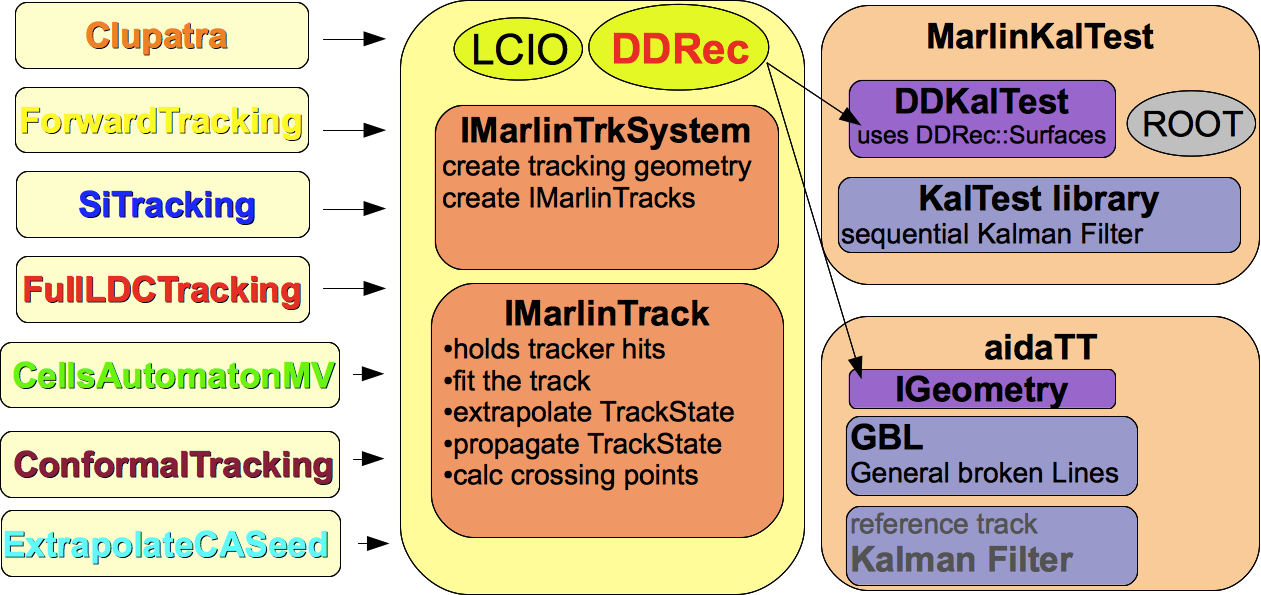
\includegraphics[width=0.80\hsize]{chapters/figures/IMarlinTrk_ddkaltest_new.png}
\end{center}
\caption{Schematic view of the MarlinTrk tracking tools available in iLCSoft. They are based on the LCIO event data model and the
DDRec geometry description.}
\label{fig:imarlintrk}
\end{figure}
%%%%%%%%%%%%%%%%%
ILD uses the following different algorithms in the different parts of the tracking region
(for more details see~\cite{Gaede:2014aza}):

\begin{itemize}
\item SiliconTracking\\
  Algorithm used in the innermost Si-tracking detector VXD and SIT, based an a brute-force triplet seeding followed by
  a road search using the extrapolation to the next layer provided in MarlinTrk.
\item ForwardTracking\\
  Stand alone pattern recognition in the FTD forward tracker using a Cellular-Automaton to find, a possibly large, set of
  track candidates that are reduced to a unique and consistent set through the use of a Hopfield Network.
\item Clupatra\\
  Pattern recognition algorithm for the TPC, based on a topological clustering in the outer TPC pad row layers for seeding,
  followed by a Kalman-Filter based road search inwards.
\item FullLDCTracking\\
  A collection of algorithms for merging track segments from the previous algorithms and assignments of leftover hits followed
  by a final re-fit using a Kalman-Filter.
\end{itemize}

SiD had originally developed their stand alone tracking software in the Java framework \emph{LCSim}~\cite{bib:LCSim}
using a triplet based seeding followed by a road search and a final track fit. More recently SiD has adopted the \emph{ConformalTracking}
algorithm originally developed for CLICdp. It uses a conformal mapping transforming circles going through the origin (IP)
into straight lines which are then identified using a Cellular-Automaton.

The correct reconstruction of the kinematics of charged particles requires a sufficiently detailed description of the material
the particles have traversed, in order to correctly account for effects of energy-loss and multiple-scattering in the fit.
The DD4hep component DDRec provides dedicated surface classes for track reconstruction and fitting. These surface classes provide the
geometric information of the corresponding measurement surfaces as well as material properties, averaged in a suitable way. Surfaces
are also used to account for effects from dead material layers, such as support structures or cables and services.


The resulting tracking efficiencies for the ILD detector are shown as a function of the momentum and
$\rm{cos}(\theta)$ in Fig~\ref{fig:ild_trkeff}.

%%%%%%%%%%%%%%%%
\begin{figure}
  \begin{tabular}[c]{c}
    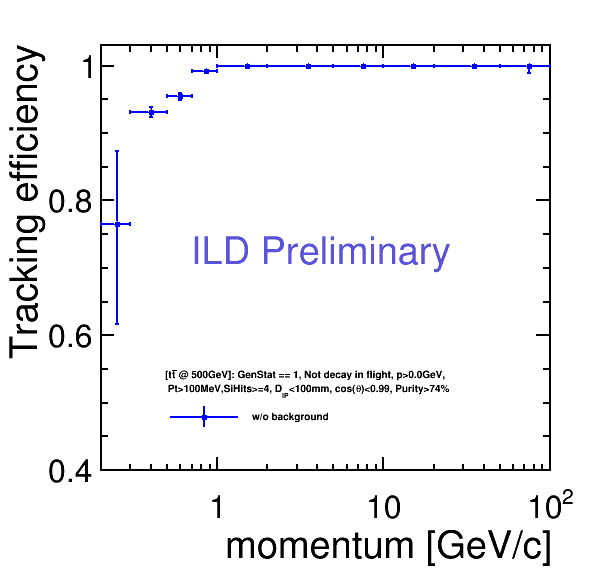
\includegraphics[width=0.85\hsize]{chapters/figures/trkEff_Momentum_ttbar_ILD_l5_v02_v02-00-02_New_publish_cuts2.png} \\
    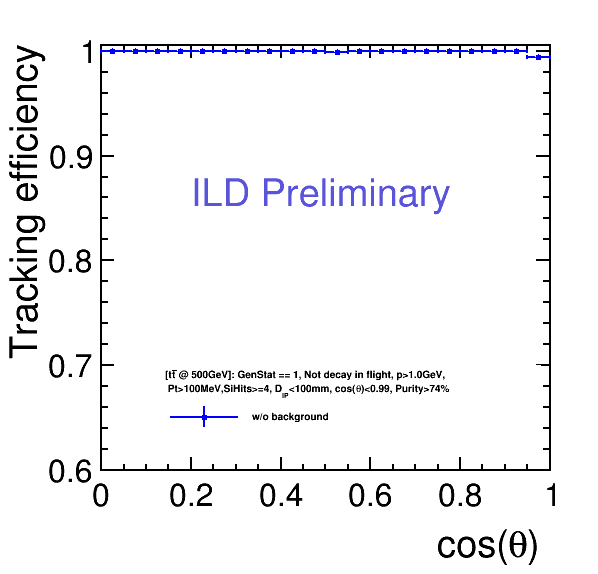
\includegraphics[width=0.85\hsize]{chapters/figures/trkEff_theta_ttbar_ILD_l5_v02_v02-00-02_New_publish_cuts1.png}
\end{tabular}
  \caption{Tracking efficiency for $t\bar t$-events at $\sqrt{s}=500~\rm{GeV}$ in the ILD detector as a function of
    momentum ($\rm{cos}(\theta)>.99$) [upper]
    and $\rm{cos}(\theta)$ ($p>1~\rm{GeV}$) [lower].}

\label{fig:ild_trkeff}
\end{figure}
%%%%%%%%%%%%%%%%%

The normalised transverse momentum resolution $\sigma(1/p_T)$ for single-muon events the SiD detector model is shown in
Fig~\ref{fig:sid_mom_res} together with fits using the parameterisation:

\begin{equation}
  \frac{\sigma(p_T)}{p^2_T} = a~\oplus~\frac{b}{p~\rm{sin}\theta}     \label{eq:trk_res_param}
\end{equation}

%%%%%%%%%%%%%%%%
\begin{figure}
\begin{center}
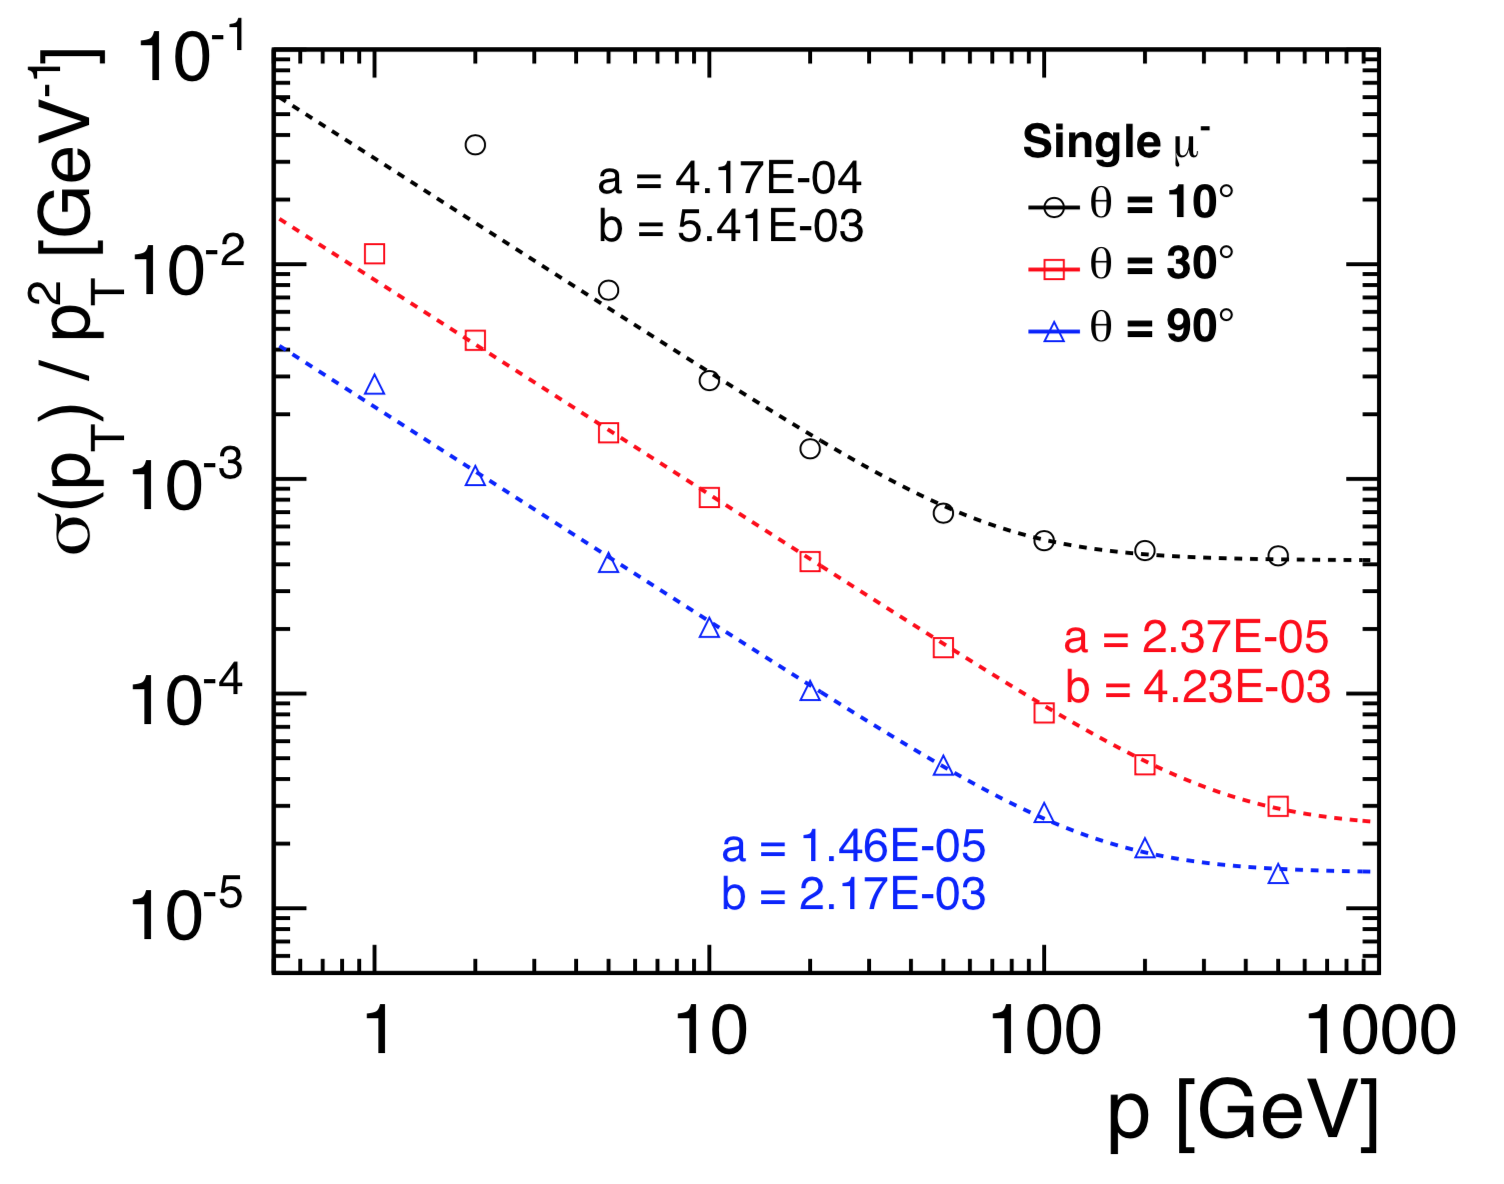
\includegraphics[width=0.95\hsize]{chapters/figures/SiD_momentum_resolution.png}
\end{center}
\caption{Normalised transverse momentum resolution for single-muon events as function of momentum
  in the \emph{SIDLOI3} simulation model (from~\cite{Behnke:2013lya}). The dashed lines are fits to the data points according
  to eq.~\ref{eq:trk_res_param}.}
\label{fig:sid_mom_res}
\end{figure}
%%%%%%%%%%%%%%%%%

Comparable results are obtained for ILD and both detector concepts achieve their design goals for the momentum resolution of
$\sigma(p_T)/P^2_T  < 2 \times 10^{-5} \rm{GeV}^{-1}$ for high momentum central tracks.

%%%%%%%%%%%%%%%%
\begin{figure}
\begin{center}
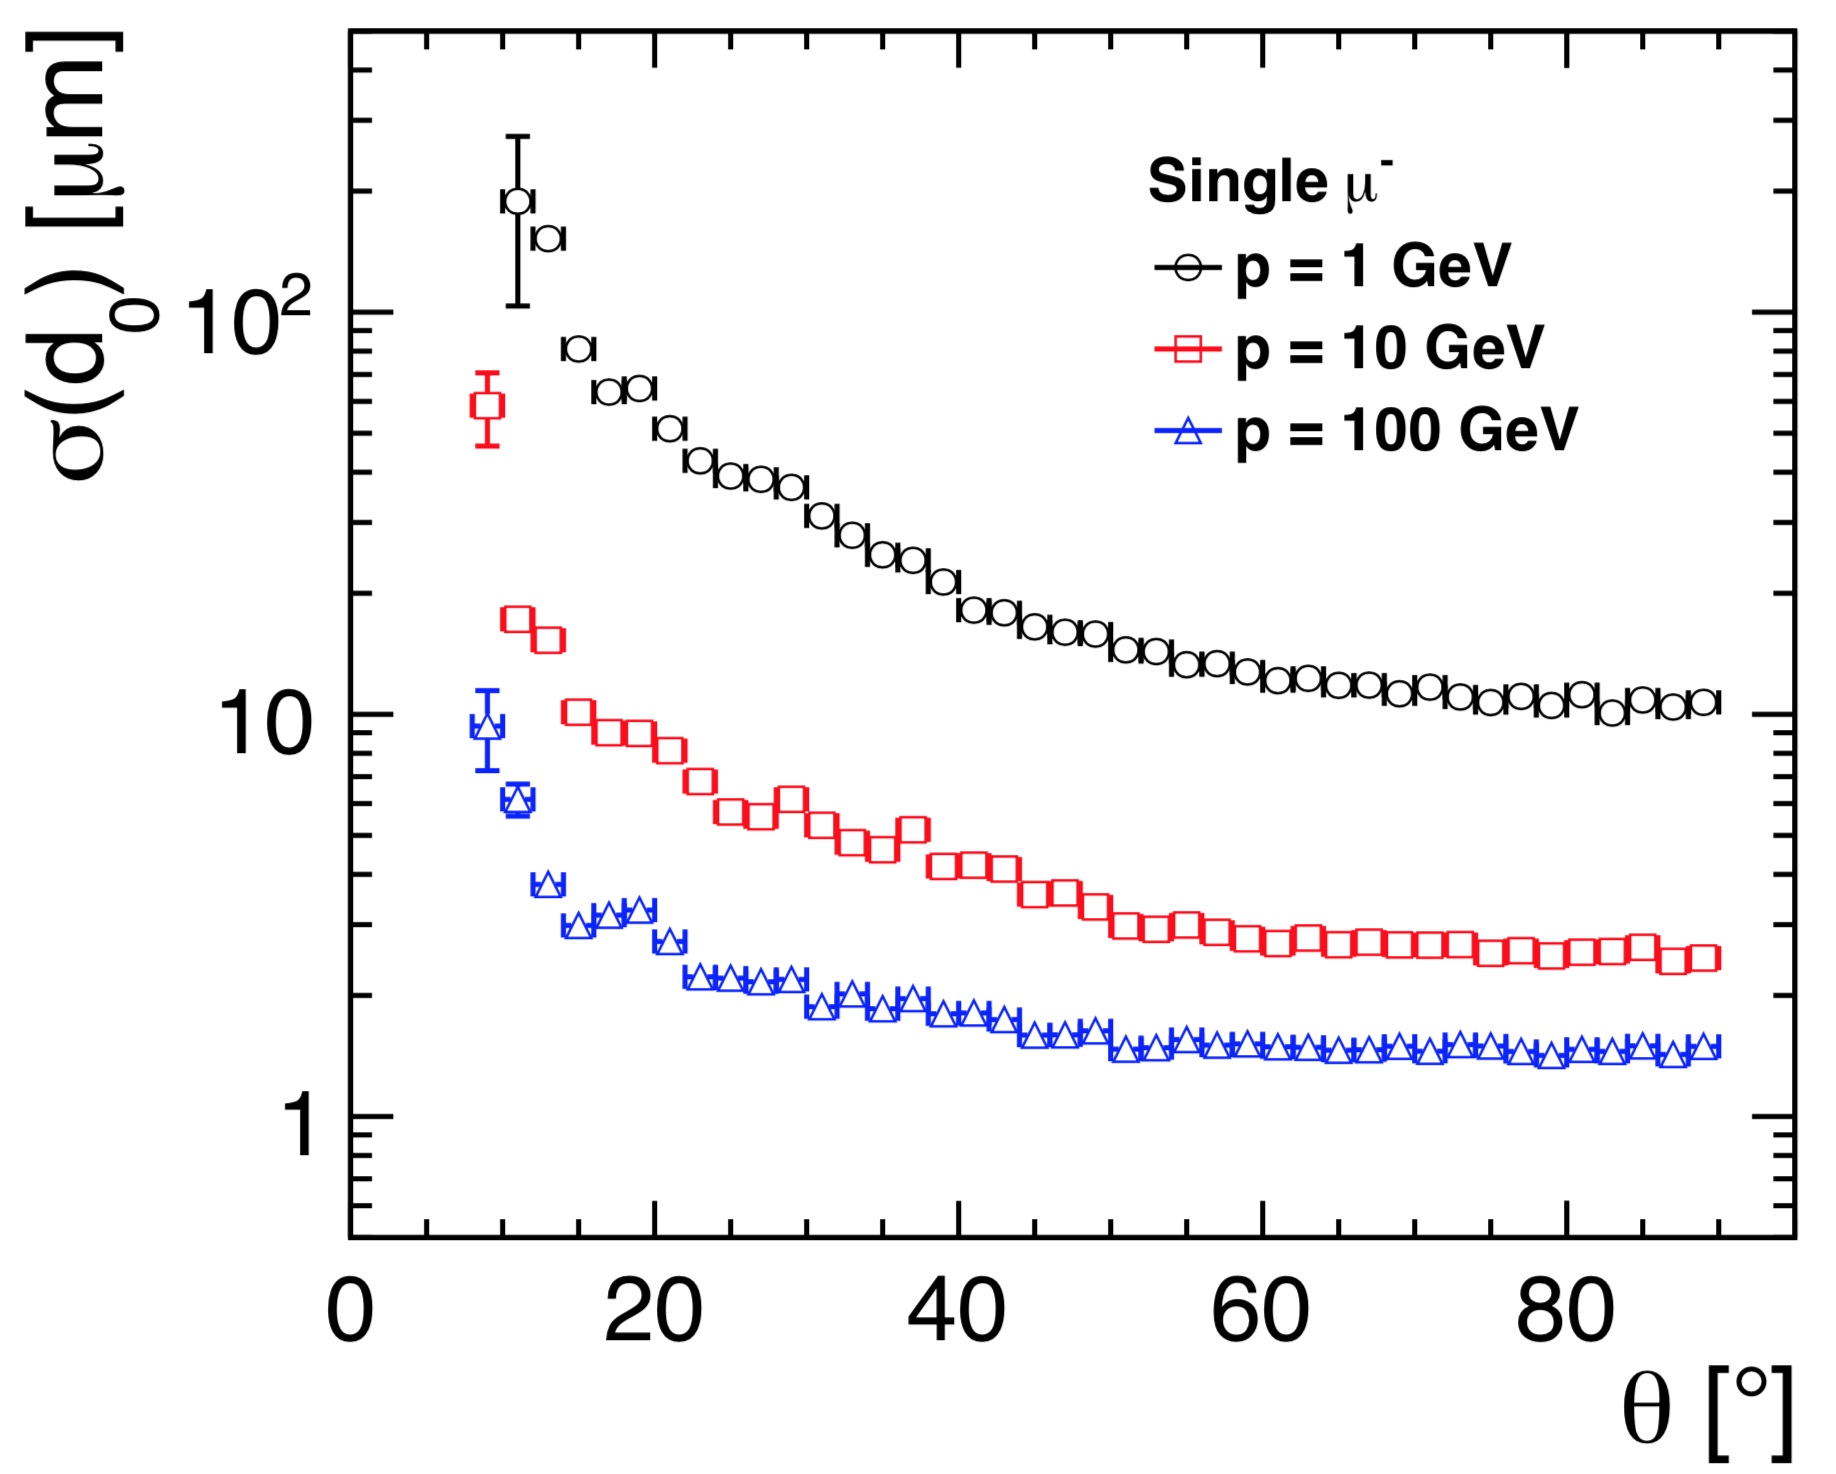
\includegraphics[width=0.85\hsize]{chapters/figures/SiD_D0_resolution.png}
\end{center}
\caption{Impact parameter resolution $\sigma(d_0)$ for single-muon events as function of polar angle
  in the \emph{SIDLOI3} simulation model (from~\cite{Behnke:2013lya}).} 
\label{fig:sid_d0_res}
\end{figure}
%%%%%%%%%%%%%%%%%

The impact paramter resolution as a function of polar angle for single-muon events in SiD is shown in Fig~\ref{fig:sid_d0_res} for
different particle momenta. A resolution of a few $\mu\rm{m}$ is achieved for high mometum tracks over a large range of the polar
angle down to $\sim 20^{o}$.


The tracking software is completed with a dedicated processors for the identification and reconstruction of kinks and $V_0$s.
Tracks with kinks can arise from bremsstrahlung, typically for electrons, or a large angle deflection due to multiple scattering.
$V_0$s are almost exclusively decays of $K^0_s$ and $\Lambda^0$ as well as gamma conversions.

%----------------------------------------------
~~~\\
Particle Flow: \\

The \emph{particle flow algorithm} (PFA) aims at reconstructing every individual particle created in the event in order
to take the best available measurement for the given particle type, i.e.:
\begin{itemize}
\item charged particles\\
  using the momentum measured in the tracking detectors with the excellent resolution described  above
\item photons\\
  measured in the Ecal with an energy resolution of $\sigma(E)/E \sim  17\% / \sqrt{(E/\rm{GeV})}$ %%\fix{is this the correct number?}
\item neutral hadrons\\
  measured predominantly in the Hcal\footnote{hadronic showers often start in the Ecal and might extend into the Muon system -
    this is taken into account in PandorPFA} with an energy resolution of $\sigma(E)/E \sim  50\% / \sqrt{(E/\rm{GeV})}$ %%\fix{is this the correct number?}
\end{itemize}

The best jet energy measurement in hadronic events would be achieved if the above algorithm would work perfectly. However in reality
there is always confusion in the assignment of individual \emph{CalorimeterHits} to Clusters and showers as well as in the assignment
of tracks to clusters. This effect is demonstrated in Fig~\ref{fig:pandorapfa_perfect} for PandoraPFA~\cite{Marshall:2015rfa}, the
implementation of PFA available in iLCSoft that is used by both detector concepts.

%%%%%%%%%%%%%%%%
\begin{figure}
\begin{center}
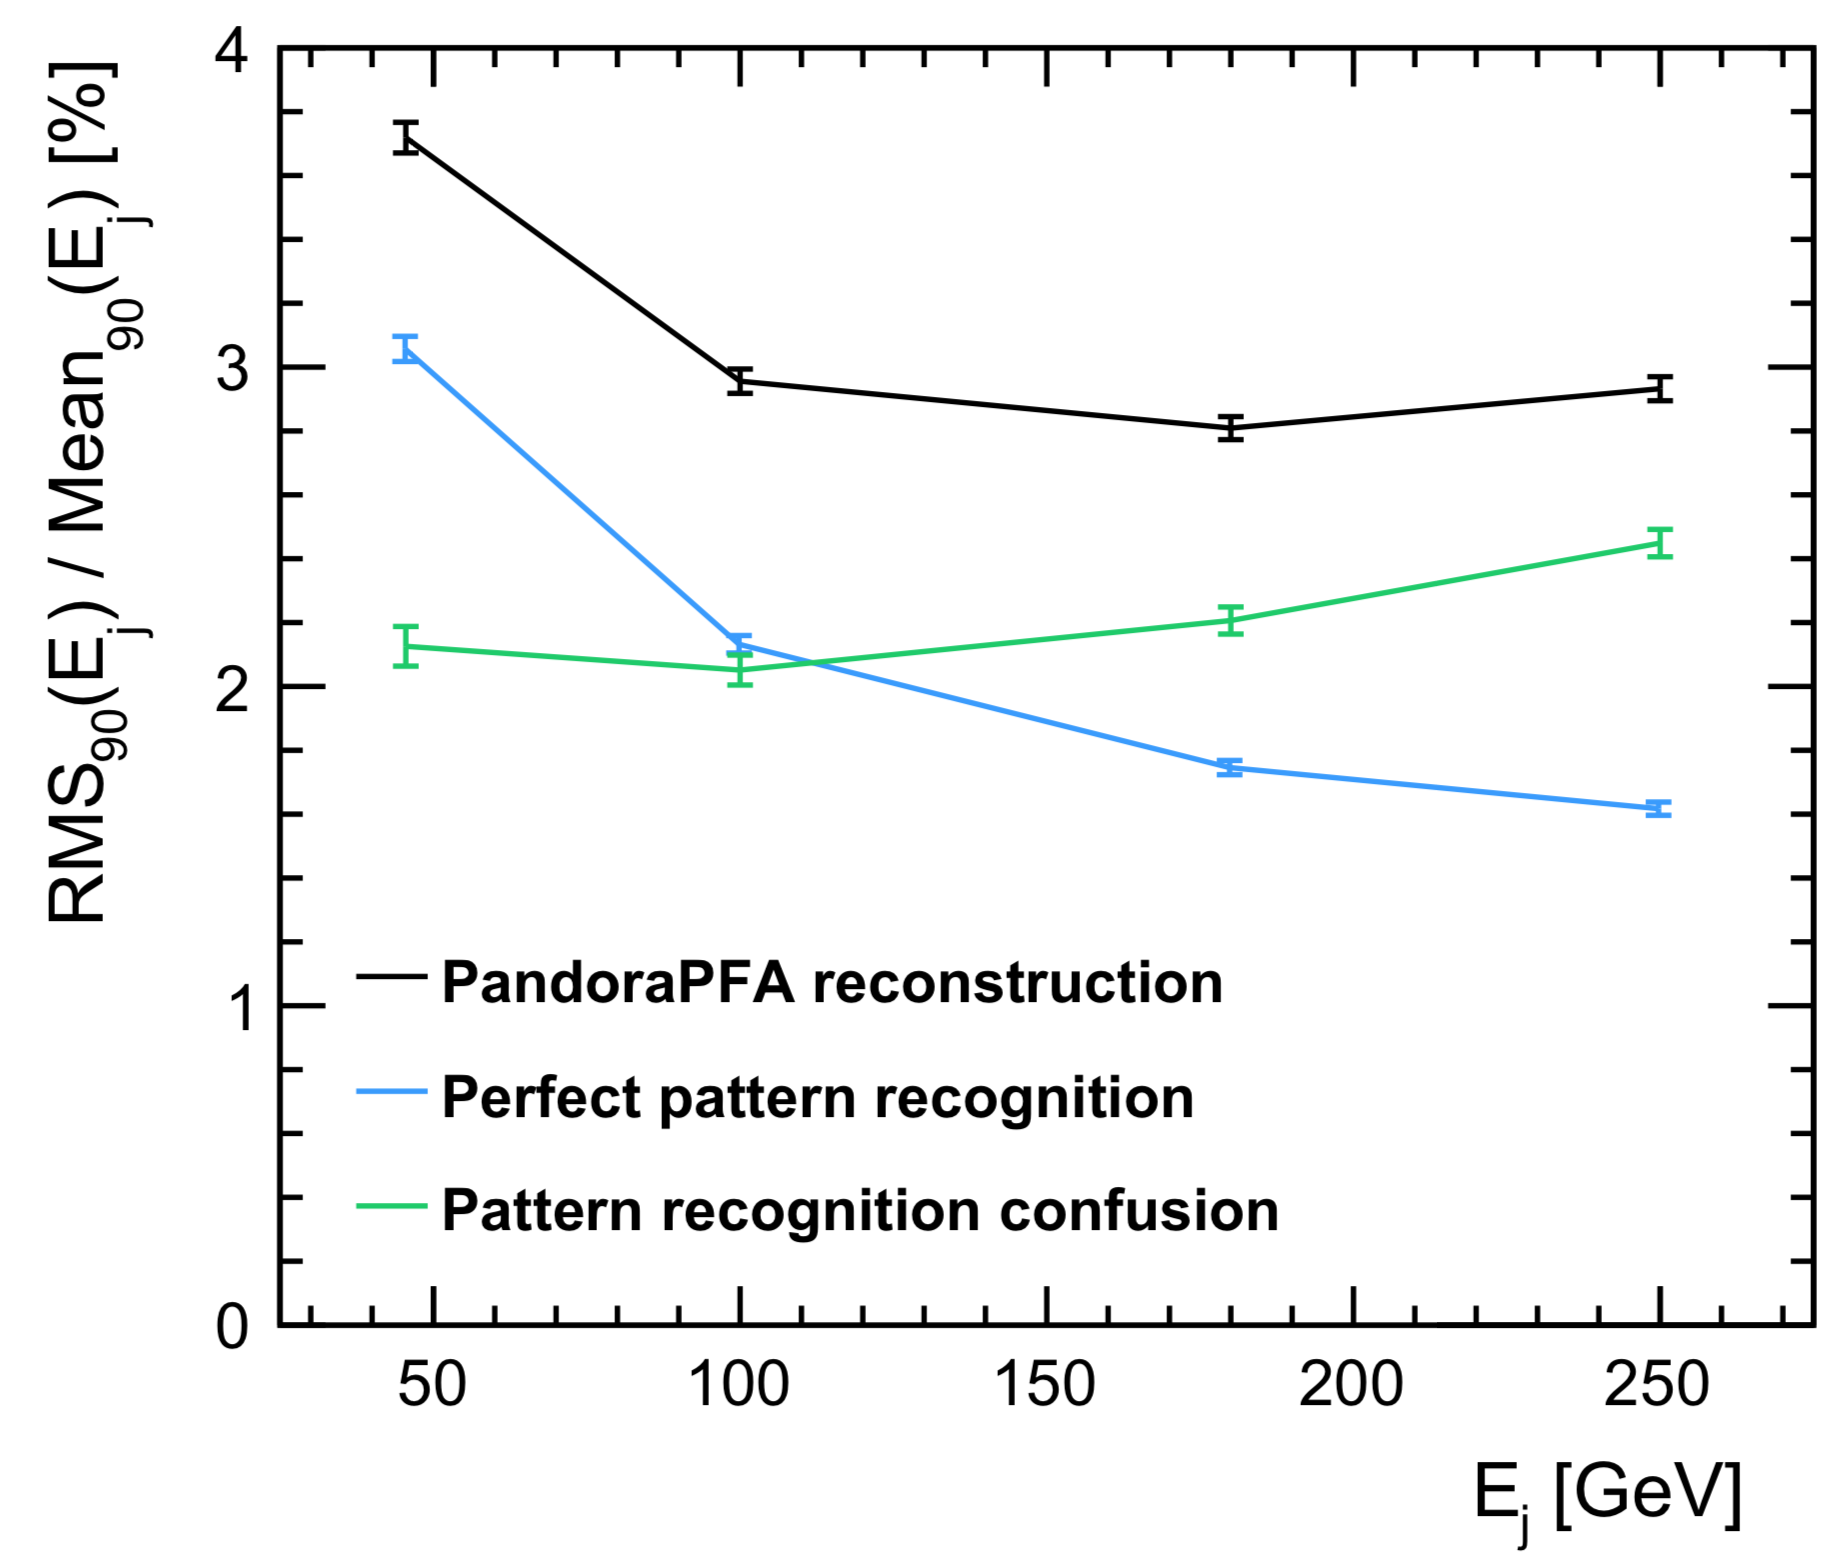
\includegraphics[width=0.85\hsize]{chapters/figures/pandorapfa_perfect.png}
\end{center}
\caption{Jet energy resolution for $Z'$ events as a function of the jet energy in a realistic detector for PandoraPFA.
  Also shown are the effect of \emph{confusion} and the result assuming \emph{perfect PFA} (from~\cite{Marshall:2015rfa}).} 
\label{fig:pandorapfa_perfect}
\end{figure}
%%%%%%%%%%%%%%%%%

The input to PandoraPFA are collections of Tracks, Kinks, $V0$s and collections of all digitized \emph{CalorimeterHits} together with
some geometrical information retrieved from DDRec.
Following~\cite{Marshall:2015rfa} the main steps of the algorithm are:

\begin{itemize}
\item \emph{CalorimeterHits} are clustered using a simple cone-based algorithm, seeded either from isolated hits in the first calorimeter
  layers or by the projection of Tracks to the front face of the Ecal.

\item the clustering algorithm is configured to prefer splitting of clusters rather than risking to falsly merge particles into single
  clusters.

\item Clusters are associated to Tracks based on topological (position and direction) and kinematic (momentum and energy) consistency.
  In case of significant discrepancies a re-clusering is initiated.

\item Clusters without associated Tracks are transformed into neutral \emph{ReconstructedParticles} unless they can be more likely
  interpreted as fragments of charged particles.
  
\item consistent Track-Cluster combinations are transformed into charged \emph{ReconstructedParticles}
  
\item particle identification plugins are applied to label specific particle types, such as photons, electrons and muons.

\item a dedicated weighting procedure known as \emph{software compensation} is applied to the hits inside a cluster in order
  to equalize hadronic and electromagnetic shower components 
  
\end{itemize}


The final output collection of PandoraPFA is called ``PandoraPFOs'' and represents the final output of the \emph{Reconstruction}
process. This collection is either directly used for physics analyses or serves as input to higher-level reconstruction
algorithms where necessary.

Fig~\ref{fig:ild_jer_jes} shows the jet energy resolution and jet energy scale that is achieved for two variants of the ILD detector
for a dedicated event sample of hadronic $Z\rightarrow u,d,s$ events.
The jet energy resolution is evaluated using $RMS_{90}(E)$, the root mean square of the energy of the central 90\% of the events.
The restriction to $u,d,s$ quarks is chosen to focus on  the detector and PFA performance without the extra complication of missing
energy due to neutrinos.

%%%%%%%%%%%%%%%%
\begin{figure}
  \begin{tabular}[c]{c}
    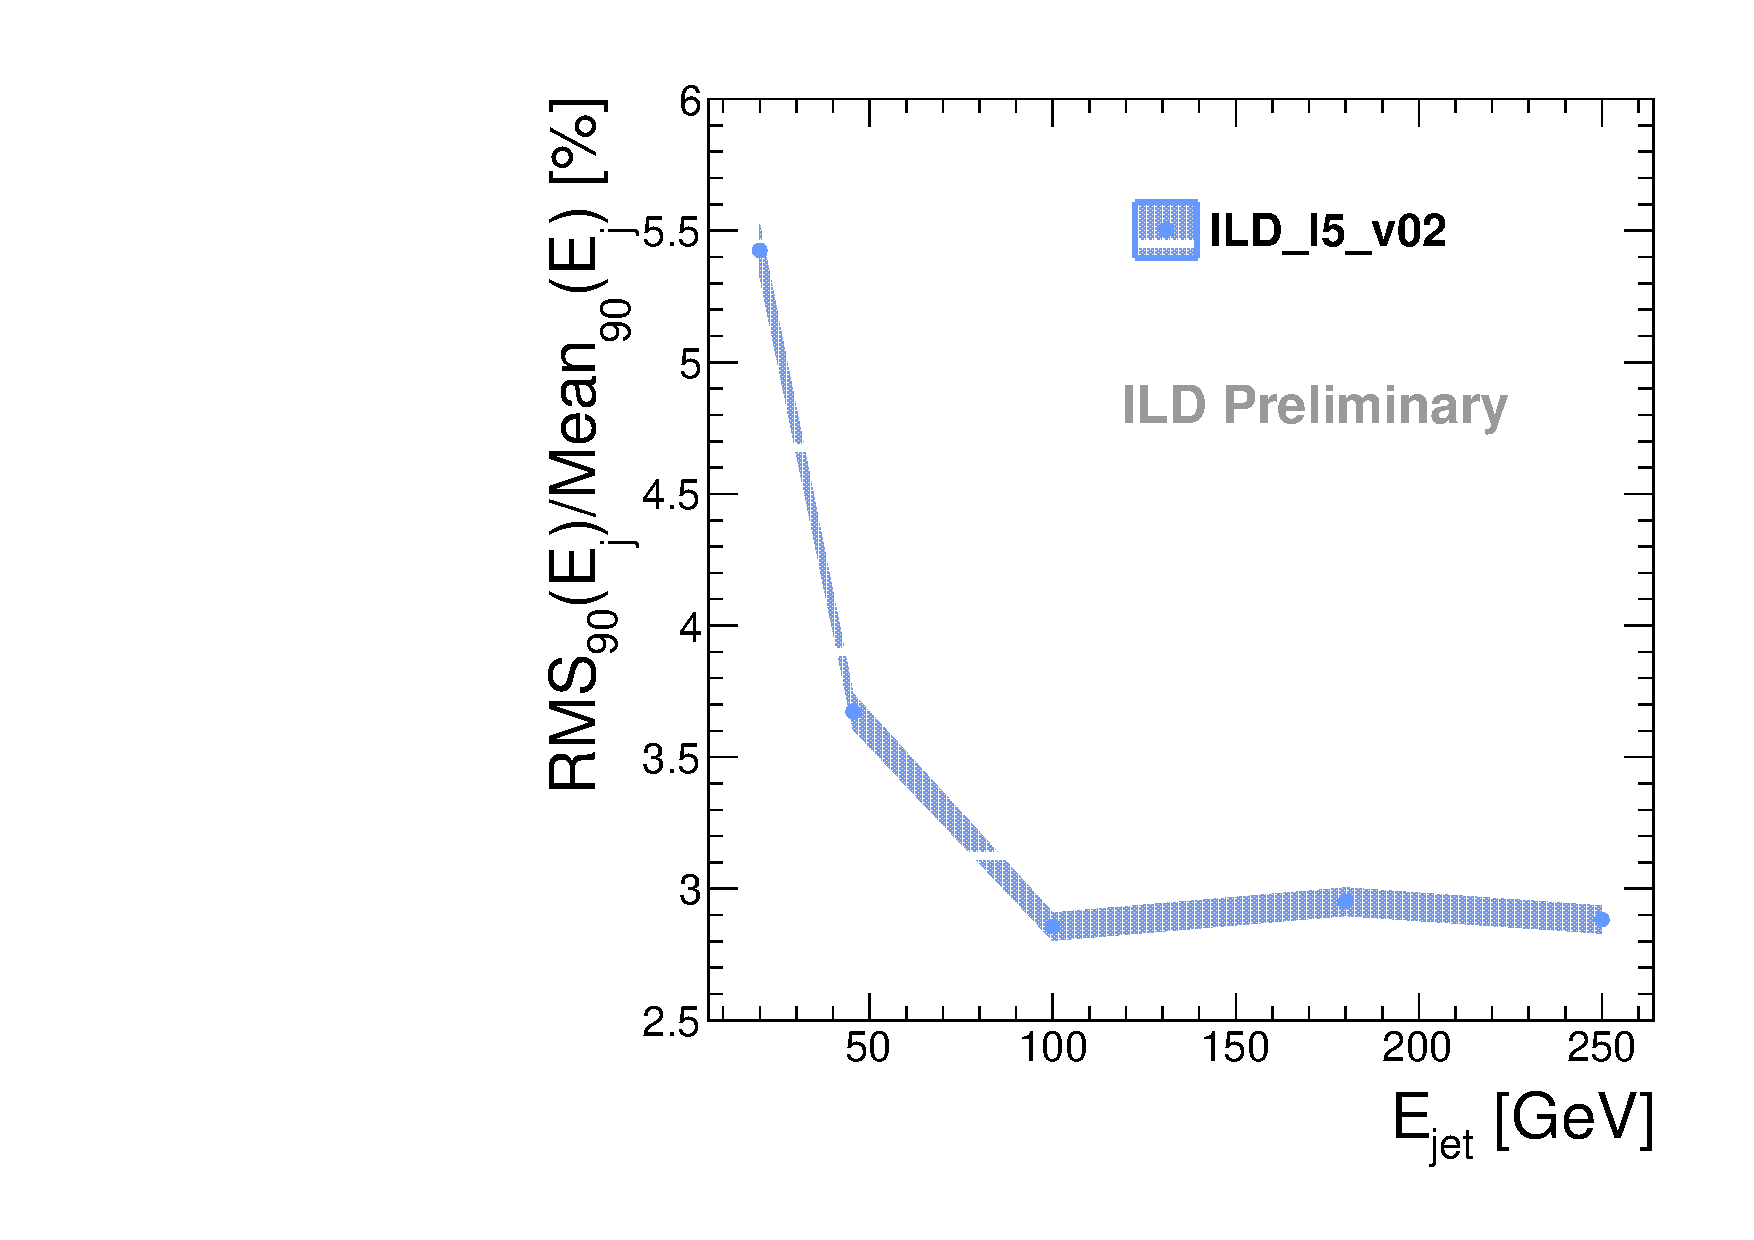
\includegraphics[width=0.85\hsize]{chapters/figures/JER_IDR_Large.pdf} \\
    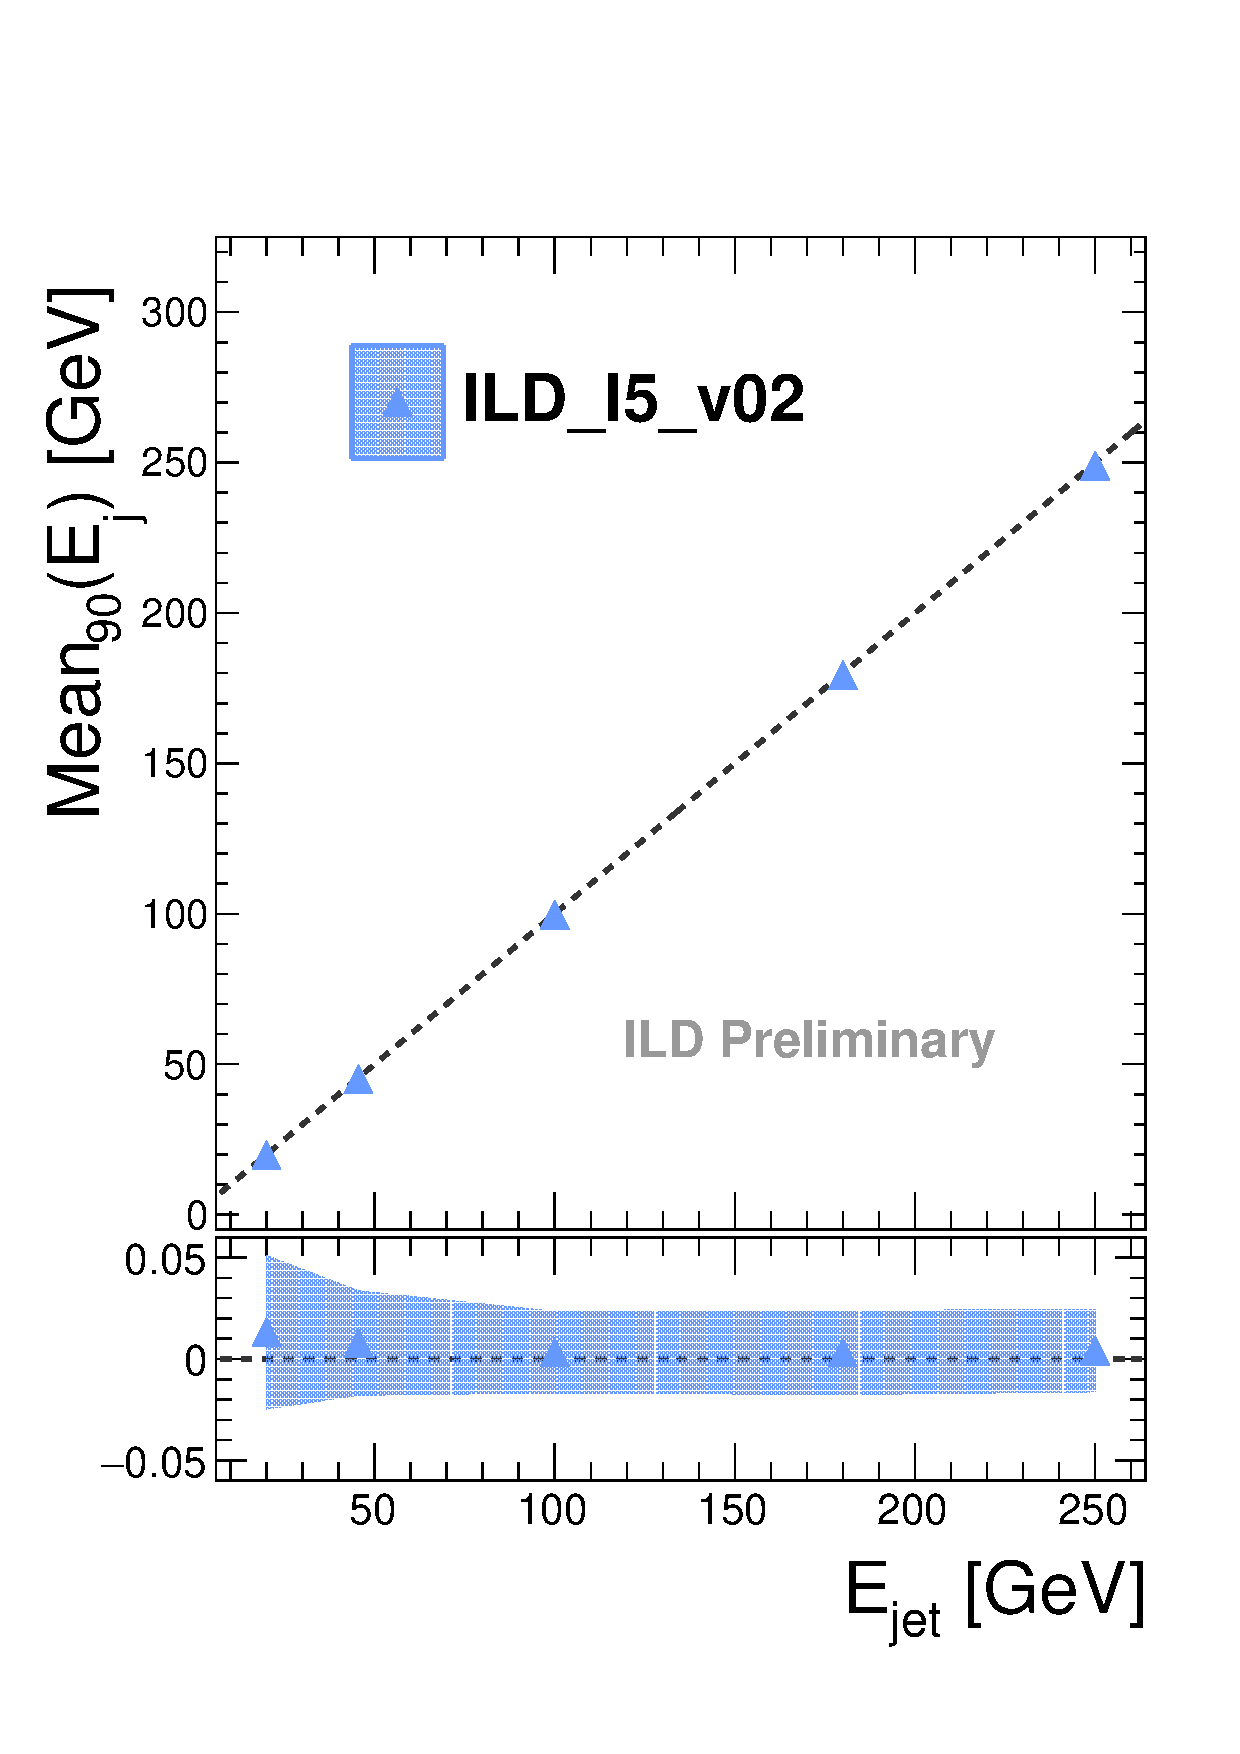
\includegraphics[width=0.85\hsize]{chapters/figures/JES_IDR_Large.pdf}
  \end{tabular}
  \caption{Upper: Jet energy resolution for $Z\rightarrow u,d,s$ events as a function of the jet energy in the standard ILD simulation model.
    Lower: The resulting jet energy scale for the same events.}
\label{fig:ild_jer_jes}
\end{figure}
%%%%%%%%%%%%%%%%%


  

%\subsubsection{High-Level Reconstruction}
\subsection{\label{sub:sw-HLR}High-Level Reconstruction}

After having reconstructed all the individual particles in the event, the next step in the processing is the reconstruction of
primary and secondary vertices. This is carried out in iLCSoft with the LCFIPlus~\cite{Suehara:2015ura} package that is also used
for the tagging of heavy flavor jets.

The primary vertex of the event is found in a tear-down procedure. First an initial vertex is fitted by a $\chi^2$-minimization using
all charged tracks in the event and a constraint from the expected beam spot
$(\sigma_x=516~\rm{nm}, \sigma_y=7.7~\rm{nm},\sigma_z \sim 200~\mu\rm{m}~~\rm{at}~~~E_{cms}=250~\rm{GeV})$.
Then all tracks with a $\chi^2$-contribution larger than a given threshold value are removed.

In a second step LCFIPlus tries to identify secondary vertices, starting out from forming all possible track-pairs from tracks not
used in the primary vertex. The pairs have to fulfill suitable requirements with respect to their invariant mass, momentum direction
and $\chi^2$. $V^0$s are excluded from these initial pairs. Secondary vertices are then formed using so far leftover tracks in
an iterative procedure and eventually adding compatible tracks originally used in the primary vertex.

Secondary vertices and optionally isolated Leptons can be used by LCFIPlus for jet clustering, aiming at high efficiency for correctly identifying
heavy flavor jets. The actual jet clustering is then performed by using a cone-based clustering with a Durham-like algorithm.
Alternatively users can use $k_T$ jet clustering algorithms from the Fastjet~\cite{Cacciari:2006sm} that is interfaced to Marlin in a dedicated
package MarlinFastJet.

LCFIPlus also provides algorithms for jet flavor tagging using boosted decision trees (BDTs) based on suitable variables from tracks and vertices.
Fig~\ref{fig:sid_flavor_tag} shows the mis-identification efficiency for jets from light quarks and c-quarks as a function of the b-tagging efficiency
for the SiD detector using LCFIPlus.

%%%%%%%%%%%%%%%%
\begin{figure}
\begin{center}
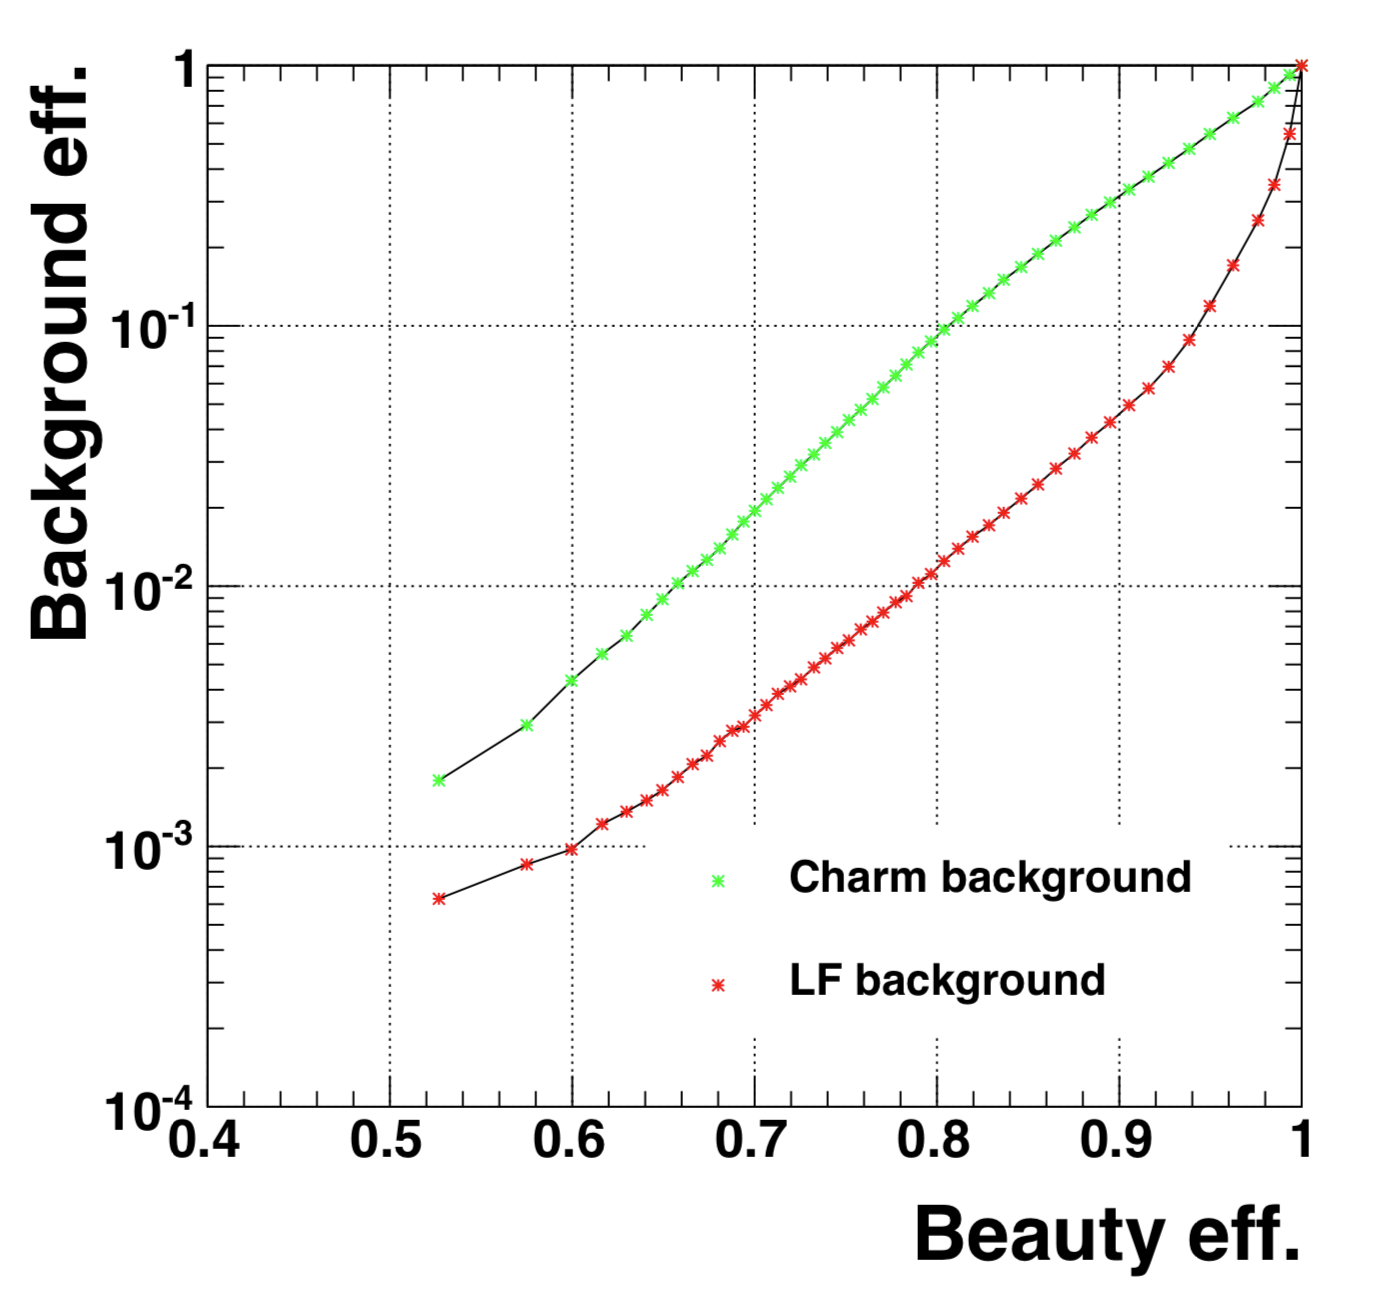
\includegraphics[width=0.9\hsize]{chapters/figures/SiD_flavor_tag.png}
\end{center}
\caption{Mis-identification efficiency of light quark jets (red points) and charm jets (green points) as beauty jets versus beauty identification efficiency in
  di-jets events at $\sqrt{s} = 91~\rm{GeV}$ (from~\cite{Behnke:2013lya}).} 
\label{fig:sid_flavor_tag}
\end{figure}
%%%%%%%%%%%%%%%%%


There is a large palette of additional high level reconstruction algorithms available in iLCSoft addressing the needs for physics analyses, e.g.
\begin{itemize}
\item particle identification using dE/dx, shower shapes and multi-variate methods
\item $\gamma\gamma$-finders for the identification of $\pi^0$s and $\eta$s
\item reconstructed particle to Monte-Carlo truth linker for cross checking analysis and reconstruction efficiencies
\item tools for jet clustering using Monte-Carlo truth information
\item processors for the computation of various event shapes 
\end{itemize}



%\subsubsection{Fast Simulation}
\subsection{\label{sub:sw-fastsim}Fast Simulation}

In addition to the full simulation and reconstruction 
outlined in the previous sections,
there is a need for simulation that can quickly generate
substantial samples of simulated and reconstructed events.
Situations were this is desirable include detector optimisation
and new physics searches. In these cases,
similar processes need to be simulated and reconstructed at
a, possibly very large, number of different conditions.
In the first case, it would amount to modifying various aspects
of the detector in steps, in the latter,
one would like to exploit the entire allowed parameter space
of a theory for new physics.
In addition to these cases,
fast simulation is also an asset for simulating high-crossection
SM processes, such as $\gamma\gamma$ processes, where the investment 
in processor power and intermediate storage might be
prohibitively large to attain the goal that simulation statistics
should be a negligible source of systematic uncertainty.

To meet these needs,
a fast simulation program needs to be fast, flexible, and
accurate. 
The SGV program\cite{Berggren:2012ar} used at ILC meets these needs.
The time to simulate and reconstruct an event is similar to
the time it takes to generated it ($\sim 1-10$~ms),
the response of the detector is as far as possible calculated
from the detector design (i.e. there is no need to parametrisise
pre-existing full simulation results),
and has been shown to well compare both with full simulation
and real data\cite{Abdallah:2003xe}.

The program uses a simplified ``{\it cylinders-and-discs}'' description
of the detector,
which is used to calculate the Kalman-filtered track-helix covariance matrix
of each generated charged particle.
By Cholesky decomposition of the covariance matrix,
the track-parameters are simulated in a way such that all correlations
are respected.
The calorimetric response is calculated from the expected single-particle
performance of the different components of the calorimetric system,
for each particle impinging on it. Optionally,
the effects of shower-confusion can be included.
To reduce the needed storage for Giga-event size sample,
event filtering can be applied at different steps of the processing,
directly after generation, after the detector response is known,
or after higher-level event analysis is done.
Events passing all filters are output in LCIO DST-format,
and can seamlessly be further analysed within the Marlin framework.


%\subsection{Computing}

%\subsubsection{Computing Concept}
\subsection{\label{sub:sw-computing}Computing Concept}


An initial computing concept for the ILC, including a first estimate of the required resources, has been developed by the LCC Software and Computing Group.

The foreseen computing concept follows in general terms that of the current LHC experiments and Belle~II, with a strong on-site computing
center complemented by large Grid-based computing resources distributed around the world. This concept is schematically shown in
Fig~\ref{fig:computing_scheme}.

%%%%%%%%%%%%%%%%
\begin{figure*}
\begin{center}
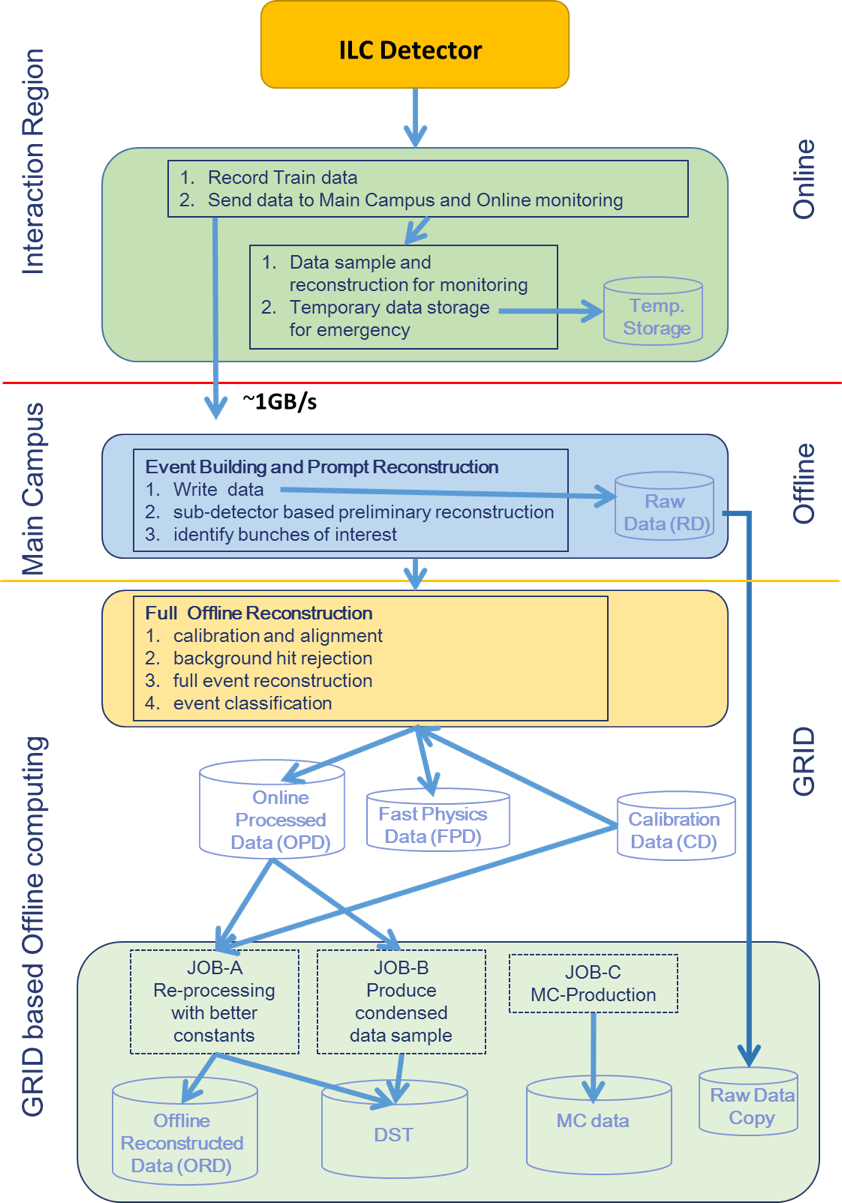
\includegraphics[width=0.6\hsize]{chapters/figures/ILC_computing_scheme.png}
\end{center}
\caption{Computing concept foreseen for the ILC, distributed over on-site computing at the interaction region, the main campus and Grid-like
  offline computing.}
\label{fig:computing_scheme}
\end{figure*}
%%%%%%%%%%%%%%%%%

Due to the much lower event rates at the ILC compared to the LHC, we will be
able to run in an un-triggered mode in which  collision data from every bunch crossing will be recorded. At the experimental site,
we require only limited computing resources for online monitoring, QA and data-buffering for a few days.

Prompt reconstruction, event building, and filtering of the interesting collisions will be performed at the main ILC campus.
A small fraction of the initial raw data will be distributed to major participating Grid sites in the world for further skimming and
final redistribution for physics analysis.
A copy of the raw data from all bunch crossings will be kept to allow  for future searches for new exotic signatures.


%\subsubsection{Resource Estimate}
\subsection{\label{sub:sw-res-estimate}Computing Resource Estimate}

Based on our detailed physics and background simulations,  we estimate the total raw data rate of the ILC to be $\sim$1.5GB/s.

The total estimated storage needs will be a few tens of PB/y.
The computing power needed for simulation, reconstruction, and analysis will be a few hundred kHepSpec06.
Given that these numbers are already smaller than what is now
needed by the LHC experiments, and given an expected annual increase
of 15\% and 20\%, respectively, for storage and CPU
at flat budget, we expect the overall computing costs for the ILC
will be more than an order of magnitude smaller than those for the LHC.

%\fix{extend this with a bit more detail, e.g. a small table with the main parameters relevant for the estimate ...}



